% SPDX-FileCopyrightText: Contributors to PyPSA-Wal
% SPDX-License-Identifier: CC-BY-4.0
%
% Compiled by workflow_onwind_wal/Snakefile (rule build_report).
% Every number in this document comes from generated/macros.tex; do not type
% figures by hand.

\documentclass[11pt,a4paper]{article}

\usepackage[T1]{fontenc}
\usepackage[utf8]{inputenc}
\usepackage[english]{babel}
\usepackage{lmodern}
\usepackage{microtype}
\usepackage[margin=2.4cm]{geometry}
\usepackage{graphicx}
\usepackage{booktabs}
\usepackage{longtable}
\usepackage{siunitx}
\usepackage{xcolor}
\usepackage{enumitem}
\usepackage{caption}
\usepackage{fancyhdr}
\usepackage[htt]{hyphenat}   % let long \texttt{} paths break across lines
\usepackage[hidelinks]{hyperref}

\emergencystretch=3em
\hyphenpenalty=1000

\sisetup{group-separator={\,},group-minimum-digits=4,detect-all}
\captionsetup{font=small,labelfont=bf}
\setlist{nosep,leftmargin=*}

\definecolor{wal}{HTML}{2B8A3E}
\definecolor{warn}{HTML}{C92A2A}
\newcommand{\finding}[1]{\par\medskip\noindent\colorbox{wal!10}{%
  \begin{minipage}{\dimexpr\linewidth-2\fboxsep}\textbf{Finding.} #1\end{minipage}}\par\medskip}
\newcommand{\caveat}[1]{\par\medskip\noindent\colorbox{warn!8}{%
  \begin{minipage}{\dimexpr\linewidth-2\fboxsep}\textbf{Caveat.} #1\end{minipage}}\par\medskip}

\pagestyle{fancy}
\fancyhf{}
\fancyhead[L]{\small Walloon onshore-wind technical potential}
\fancyhead[R]{\small PyPSA-Wal}
\fancyfoot[C]{\thepage}
\renewcommand{\headrulewidth}{0.3pt}

\newcommand{\refScenario}{S6\_servitudes}
\newcommand{\refScenarioTitle}{+ aeronautical servitudes, slope $\geq$ 7 \%, classified sites, radar}
\newcommand{\refTurbine}{NREL 2020ATB 4.0 MW (tip 185 m)}
\newcommand{\refDensity}{5.08}
\newcommand{\adminArea}{16\,905}
\newcommand{\modelArea}{15\,150}
\newcommand{\modelCoverage}{89.6}
\newcommand{\areaOutsideModel}{2\,191}
\newcommand{\areaOutsideWallonia}{435}
\newcommand{\AdminEligible}{420}
\newcommand{\AdminEligibleShare}{2.49}
\newcommand{\AdminPnom}{2\,136}
\newcommand{\AdminPnomGW}{2.14}
\newcommand{\AdminFlh}{3\,260}
\newcommand{\AdminEnergy}{6.96}
\newcommand{\AdminTurbines}{534}
\newcommand{\PlaceModel}{parks+horizon}
\newcommand{\PlaceLink}{1.5}
\newcommand{\PlaceMinTurbines}{4}
\newcommand{\PlaceAzimuth}{130}
\newcommand{\PlaceHorizonRadius}{4}
\newcommand{\MotorwayExempt}{1}
\newcommand{\PlaceParks}{453}
\newcommand{\PlacePerPark}{4.5}
\newcommand{\PlaceMedianPark}{2}
\newcommand{\PlaceLargestPark}{55}
\newcommand{\PlaceRotorD}{5.0}
\newcommand{\PlaceRefused}{25\,940}
\newcommand{\PlaceCheckSpacing}{762}
\newcommand{\PlaceCheckArc}{130.0}
\newcommand{\NoHorizonPnom}{11\,084}
\newcommand{\NoHorizonParks}{611}
\newcommand{\NoHorizonTurbines}{2\,771}
\newcommand{\HorizonCostPct}{26}
\newcommand{\ParksCostPct}{3}
\newcommand{\ParksFourPnom}{6\,480}
\newcommand{\ParksFourParks}{168}
\newcommand{\ParksFourTurbines}{1\,620}
\newcommand{\SmallGroupsGainPct}{26}
\newcommand{\PlaceSmallShare}{20.7}
\newcommand{\PlaceSingleShare}{8.4}
\newcommand{\FreePnom}{11\,460}
\newcommand{\FreePnomGW}{11.5}
\newcommand{\FreeTurbines}{2\,865}
\newcommand{\FreeDensity}{27.4}
\newcommand{\FreeOrderSpread}{14}
\newcommand{\ShareOfFree}{71}
\newcommand{\FreeOverRef}{1.40}
\newcommand{\IdFourMW}{6\,316}
\newcommand{\IdFourParks}{284}
\newcommand{\IdFourTurbines}{1\,579}
\newcommand{\IdSixMW}{4\,892}
\newcommand{\IdSixParks}{193}
\newcommand{\IdSixTurbines}{1\,223}
\newcommand{\SpObsD}{4.3}
\newcommand{\SpObsFree}{12\,852}
\newcommand{\SpObsMW}{9\,120}
\newcommand{\SpCrossD}{5.0}
\newcommand{\SpCrossFree}{11\,460}
\newcommand{\SpCrossMW}{8\,172}
\newcommand{\SpIsoD}{5.9}
\newcommand{\SpIsoFree}{9\,912}
\newcommand{\SpIsoMW}{7\,076}
\newcommand{\InterdistLow}{3\,742}
\newcommand{\InterdistHigh}{4\,832}
\newcommand{\PlaceSpacing}{750}
\newcommand{\PlaceTurbines}{2\,043}
\newcommand{\PlacePnom}{8\,172}
\newcommand{\PlacePnomGW}{8.2}
\newcommand{\PlaceDensity}{19.55}
\newcommand{\PlaceEnergy}{26.64}
\newcommand{\PlaceVsDensity}{283}
\newcommand{\PlaceRangeLow}{8\,172}
\newcommand{\PlaceRangeHigh}{9\,493}
\newcommand{\PlaceVOneTwelve}{8\,802}
\newcommand{\FreeVOneTwelve}{12\,342}
\newcommand{\PlaceNRELFour}{8\,172}
\newcommand{\FreeNRELFour}{11\,460}
\newcommand{\PlaceNRELFive}{9\,493}
\newcommand{\FreeNRELFive}{13\,052}
\newcommand{\ResSurvival}{76}
\newcommand{\ResCentral}{6\,252}
\newcommand{\ResCentralGW}{6.3}
\newcommand{\ResCentralEnergy}{20.38}
\newcommand{\ResLow}{4\,576}
\newcommand{\ResHigh}{8\,172}
\newcommand{\ResOrnithology}{10}
\newcommand{\ResPartial}{15}
\newcommand{\CredibleLow}{4\,576}
\newcommand{\CredibleHigh}{8\,172}
\newcommand{\CredibleLowGW}{4.6}
\newcommand{\CredibleHighGW}{8.2}
\newcommand{\CredibleCentral}{6\,252}
\newcommand{\DeDensity}{178}
\newcommand{\DeTurbines}{80.3}
\newcommand{\WalDensityToday}{90}
\newcommand{\WalDensityCentral}{370}
\newcommand{\WalDensityHigh}{483}
\newcommand{\CentralVsDe}{2.08}
\newcommand{\HighVsDe}{2.72}
\newcommand{\TodayVsDe}{0.51}
\newcommand{\CredibleCentralGW}{6.3}
\newcommand{\FleetN}{652}
\newcommand{\FleetNatureRatio}{0.01}
\newcommand{\FleetNaturePct}{0.2}
\newcommand{\FleetNatureCond}{0.00}
\newcommand{\FleetNatureCondPct}{0.0}
\newcommand{\FleetNatureCondLand}{3.8}
\newcommand{\FleetSlopeRatio}{0.15}
\newcommand{\FleetSlopePct}{5.5}
\newcommand{\FleetSlopeCond}{0.15}
\newcommand{\FleetSlopeCondPct}{3.7}
\newcommand{\FleetSlopeCondLand}{24.6}
\newcommand{\FleetAviationRatio}{0.20}
\newcommand{\FleetAviationPct}{1.5}
\newcommand{\FleetAviationCond}{0.12}
\newcommand{\FleetAviationCondPct}{1.5}
\newcommand{\FleetAviationCondLand}{12.1}
\newcommand{\FleetHabitatRatio}{0.38}
\newcommand{\FleetHabitatPct}{23.3}
\newcommand{\FleetHabitatCond}{0.31}
\newcommand{\FleetHabitatCondPct}{22.2}
\newcommand{\FleetHabitatCondLand}{71.6}
\newcommand{\FleetDwellingRatio}{0.20}
\newcommand{\FleetDwellingPct}{12.3}
\newcommand{\FleetDwellingCond}{0.14}
\newcommand{\FleetDwellingCondPct}{9.7}
\newcommand{\FleetDwellingCondLand}{69.4}
\newcommand{\FleetRiskRatio}{0.32}
\newcommand{\FleetRiskPct}{3.5}
\newcommand{\FleetRiskCond}{0.51}
\newcommand{\FleetRiskCondPct}{4.6}
\newcommand{\FleetRiskCondLand}{9.1}
\newcommand{\FleetInfraRatio}{0.83}
\newcommand{\FleetInfraPct}{11.5}
\newcommand{\FleetInfraCond}{0.61}
\newcommand{\FleetInfraCondPct}{12.1}
\newcommand{\FleetInfraCondLand}{19.7}
\newcommand{\FleetZoningRatio}{0.33}
\newcommand{\FleetZoningPct}{20.7}
\newcommand{\FleetZoningCond}{0.38}
\newcommand{\FleetZoningCondPct}{20.2}
\newcommand{\FleetZoningCondLand}{53.1}
\newcommand{\FleetLandscapeRatio}{0.17}
\newcommand{\FleetLandscapePct}{5.5}
\newcommand{\FleetLandscapeCond}{0.23}
\newcommand{\FleetLandscapeCondPct}{4.4}
\newcommand{\FleetLandscapeCondLand}{19.1}
\newcommand{\FleetLandscapePdsRatio}{0.04}
\newcommand{\FleetLandscapePdsPct}{0.8}
\newcommand{\FleetLandscapePdsCond}{0.04}
\newcommand{\FleetLandscapePdsCondPct}{0.2}
\newcommand{\FleetLandscapePdsCondLand}{5.7}
\newcommand{\FleetLandscapeAdesaRatio}{0.24}
\newcommand{\FleetLandscapeAdesaPct}{5.1}
\newcommand{\FleetLandscapeAdesaCond}{0.25}
\newcommand{\FleetLandscapeAdesaCondPct}{4.1}
\newcommand{\FleetLandscapeAdesaCondLand}{16.6}
\newcommand{\FleetHeritageRatio}{0.08}
\newcommand{\FleetHeritagePct}{0.2}
\newcommand{\FleetHeritageCond}{0.00}
\newcommand{\FleetHeritageCondPct}{0.0}
\newcommand{\FleetHeritageCondLand}{0.5}
\newcommand{\FleetRadarRatio}{0.00}
\newcommand{\FleetRadarPct}{0.0}
\newcommand{\FleetRadarCond}{0.00}
\newcommand{\FleetRadarCondPct}{0.0}
\newcommand{\FleetRadarCondLand}{0.8}
\newcommand{\FleetMaxRatio}{0.83}
\newcommand{\FleetMaxCond}{0.61}
\newcommand{\FleetSOnePct}{79}
\newcommand{\FleetSTwoPct}{50}
\newcommand{\FleetSThreePct}{50}
\newcommand{\FleetSFourPct}{48}
\newcommand{\FleetSFivePct}{46}
\newcommand{\FleetSSixPct}{44}
\newcommand{\FleetRefPct}{44}
\newcommand{\FleetRefN}{287}
\newcommand{\FleetZoningCodt}{79}
\newcommand{\FleetZoningPsroads}{86}
\newcommand{\FleetZoningNocorridor}{96}
\newcommand{\FleetFarms}{134}
\newcommand{\FleetPerFarm}{4.9}
\newcommand{\FleetFarmsFour}{72}
\newcommand{\FleetLargestFarm}{27}
\newcommand{\FleetFarmLink}{1.5}
\newcommand{\FleetInBigFarms}{86}
\newcommand{\FleetFarmsOne}{42}
\newcommand{\FleetFarmsTwo}{13}
\newcommand{\FleetFarmsThree}{7}
\newcommand{\FleetFarmsSmall}{62}
\newcommand{\FleetInSmallFarms}{89}
\newcommand{\FleetInSmallFarmsPct}{13.7}
\newcommand{\FleetSinglePct}{6.4}
\newcommand{\FleetSmallAgri}{56}
\newcommand{\FleetSmallZae}{17}
\newcommand{\FleetSmallOther}{16}
\newcommand{\FleetForestN}{10}
\newcommand{\FleetForestCodt}{1}
\newcommand{\FleetForestConif}{7}
\newcommand{\FleetForestAll}{10}
\newcommand{\FleetForestFarms}{4}
\newcommand{\FleetMachineNNPFive}{278}
\newcommand{\FleetMachineNNPTen}{306}
\newcommand{\FleetMachineNNPTwentyFive}{362}
\newcommand{\FleetMachineNNPFifty}{427}
\newcommand{\FleetMachineNNPSeventyFive}{517}
\newcommand{\FleetMachineNNPNinety}{690}
\newcommand{\FleetFarmRadPFive}{179}
\newcommand{\FleetFarmRadPTen}{228}
\newcommand{\FleetFarmRadPTwentyFive}{478}
\newcommand{\FleetFarmRadPFifty}{815}
\newcommand{\FleetFarmRadPSeventyFive}{1\,308}
\newcommand{\FleetFarmRadPNinety}{1\,561}
\newcommand{\FleetFarmEdgePFive}{1\,554}
\newcommand{\FleetFarmEdgePTen}{1\,584}
\newcommand{\FleetFarmEdgePTwentyFive}{2\,042}
\newcommand{\FleetFarmEdgePFifty}{3\,798}
\newcommand{\FleetFarmEdgePSeventyFive}{6\,680}
\newcommand{\FleetFarmEdgePNinety}{9\,091}
\newcommand{\FleetEdgeBelowFour}{53}
\newcommand{\FleetEdgeBelowSix}{69}
\newcommand{\FleetMwFarms}{47}
\newcommand{\FleetNonMwEdgeBelowFour}{39}
\newcommand{\FleetNearMotorway}{34}
\newcommand{\FleetNearMotorwayWide}{37}
\newcommand{\FleetAddrN}{134}
\newcommand{\FleetAddrZae}{65}
\newcommand{\FleetAddrAgri}{36}
\newcommand{\HorizonSettlements}{2\,261}
\newcommand{\HorizonAffected}{880}
\newcommand{\HorizonAffectedPct}{39}
\newcommand{\HorizonFailing}{6}
\newcommand{\HorizonFailingPct}{0.7}
\newcommand{\HorizonArcPOne}{152}
\newcommand{\HorizonArcPFive}{180}
\newcommand{\HorizonArcPFifty}{334}
\newcommand{\SensReferenceMW}{8\,172}
\newcommand{\SensReferencePct}{0}
\newcommand{\SensReferenceArea}{418}
\newcommand{\SensReferenceFree}{11\,460}
\newcommand{\SensIdFourMW}{6\,316}
\newcommand{\SensIdFourPct}{$-$23}
\newcommand{\SensIdFourArea}{418}
\newcommand{\SensIdFourFree}{11\,460}
\newcommand{\SensIdSixMW}{4\,892}
\newcommand{\SensIdSixPct}{$-$40}
\newcommand{\SensIdSixArea}{418}
\newcommand{\SensIdSixFree}{11\,460}
\newcommand{\SensNoHorizonMW}{11\,084}
\newcommand{\SensNoHorizonPct}{+36}
\newcommand{\SensNoHorizonArea}{418}
\newcommand{\SensNoHorizonFree}{11\,460}
\newcommand{\SensParksFourMW}{6\,480}
\newcommand{\SensParksFourPct}{$-$21}
\newcommand{\SensParksFourArea}{418}
\newcommand{\SensParksFourFree}{11\,460}
\newcommand{\SensNoCorridorMW}{10\,772}
\newcommand{\SensNoCorridorPct}{+32}
\newcommand{\SensNoCorridorArea}{667}
\newcommand{\SensNoCorridorFree}{16\,728}
\newcommand{\SensHabitatOldMW}{6\,408}
\newcommand{\SensHabitatOldPct}{$-$22}
\newcommand{\SensHabitatOldArea}{279}
\newcommand{\SensHabitatOldFree}{8\,256}
\newcommand{\SensNoAdesaMW}{8\,992}
\newcommand{\SensNoAdesaPct}{+10}
\newcommand{\SensNoAdesaArea}{480}
\newcommand{\SensNoAdesaFree}{12\,984}
\newcommand{\SensNoLandscapeMW}{9\,356}
\newcommand{\SensNoLandscapePct}{+14}
\newcommand{\SensNoLandscapeArea}{507}
\newcommand{\SensNoLandscapeFree}{13\,832}
\newcommand{\SensSlopeTenMW}{8\,712}
\newcommand{\SensSlopeTenPct}{+7}
\newcommand{\SensSlopeTenArea}{487}
\newcommand{\SensSlopeTenFree}{12\,256}
\newcommand{\SensSlopeFifteenMW}{8\,996}
\newcommand{\SensSlopeFifteenPct}{+10}
\newcommand{\SensSlopeFifteenArea}{524}
\newcommand{\SensSlopeFifteenFree}{12\,696}
\newcommand{\SensNoAviationMW}{8\,980}
\newcommand{\SensNoAviationPct}{+10}
\newcommand{\SensNoAviationArea}{484}
\newcommand{\SensNoAviationFree}{12\,656}
\newcommand{\SensForestConifMW}{10\,988}
\newcommand{\SensForestConifPct}{+34}
\newcommand{\SensForestConifArea}{615}
\newcommand{\SensForestConifFree}{15\,344}
\newcommand{\SensForestAllMW}{14\,024}
\newcommand{\SensForestAllPct}{+72}
\newcommand{\SensForestAllArea}{954}
\newcommand{\SensForestAllFree}{20\,568}
\newcommand{\SensPicPdsMW}{10\,028}
\newcommand{\SensPicPdsPct}{+23}
\newcommand{\SensPicPdsArea}{557}
\newcommand{\SensPicPdsFree}{14\,728}
\newcommand{\SensRelaxedMW}{13\,368}
\newcommand{\SensRelaxedPct}{+64}
\newcommand{\SensRelaxedArea}{862}
\newcommand{\SensRelaxedFree}{20\,176}
\newcommand{\SensTightenedMW}{4\,336}
\newcommand{\SensTightenedPct}{$-$47}
\newcommand{\SensTightenedArea}{418}
\newcommand{\SensTightenedFree}{11\,460}
\newcommand{\ServBase}{621}
\newcommand{\ServCombined}{418}
\newcommand{\ServCombinedRemoved}{203}
\newcommand{\ServCombinedPct}{33}
\newcommand{\ServAviationRemoved}{71}
\newcommand{\ServAviationPct}{11.4}
\newcommand{\ServSlopeRemoved}{128}
\newcommand{\ServSlopePct}{20.6}
\newcommand{\ServHeritageRemoved}{2}
\newcommand{\ServHeritagePct}{0.4}
\newcommand{\ServRadarRemoved}{9}
\newcommand{\ServRadarPct}{1.4}
\newcommand{\BaseEligible}{3\,757}
\newcommand{\BasePnom}{19\,079}
\newcommand{\BasePnomGW}{19.1}
\newcommand{\CapToday}{6\,500}
\newcommand{\CapTodayGW}{6.5}
\newcommand{\Installed}{1\,528}
\newcommand{\TargetGWh}{6\,200}
\newcommand{\TargetTWh}{6.2}
\newcommand{\SpwNewGWh}{3\,959}
\newcommand{\SpwNewTWh}{3.96}
\newcommand{\SpwStrictArea}{175}
\newcommand{\SpwEnlargedArea}{272}
\newcommand{\BregTotal}{11\,400}
\newcommand{\BregTotalGW}{11.4}
\newcommand{\BregCurrent}{1\,010}
\newcommand{\BregAdditional}{10\,390}
\newcommand{\BregEnergy}{18.2}
\newcommand{\BregFlh}{1\,586}
\newcommand{\BregFlhGross}{2\,298}
\newcommand{\BregPerf}{0.69}
\newcommand{\BregEmuArea}{1\,034}
\newcommand{\BregEmuMW}{25\,087}
\newcommand{\BregEmuGW}{25.1}
\newcommand{\BregEmuGrossMW}{25\,087}
\newcommand{\BregReportedShare}{45}
\newcommand{\BregBridgeEndMW}{13\,309}
\newcommand{\BregBridgeEndArea}{453}
\newcommand{\BregVsFree}{0.99}
\newcommand{\BregVsReference}{1.4}
\newcommand{\BregVsCentral}{1.8}
\newcommand{\HabitatSetback}{592}
\newcommand{\HabitatRule}{cdr2024}
\newcommand{\DwellingSetback}{400}
\newcommand{\RoadSetback}{112}
\newcommand{\RailSetback}{50}
\newcommand{\HslSetback}{190}
\newcommand{\HslKm}{312}
\newcommand{\HvSetback}{225}
\newcommand{\AddrPoints}{1\,512\,246}
\newcommand{\AddrExempt}{18\,721}
\newcommand{\PicMotorwayKm}{729}
\newcommand{\PicDualKm}{3\,171}
\newcommand{\PdsRoadKm}{6\,128}
\newcommand{\KarstKept}{131}
\newcommand{\KarstTotal}{449}
\newcommand{\TipHeight}{185}
\newcommand{\RotorDiameter}{150}
\newcommand{\HabitatSetbackVOneTwelve}{568}
\newcommand{\ValFlh}{2\,442}
\newcommand{\ValArea}{3\,757}
\newcommand{\ValCf}{27.9}
\newcommand{\ValRefFlh}{2\,425}
\newcommand{\ValDelta}{0.7}
\newcommand{\VOneTwelveFlh}{2\,467}
\newcommand{\CapRatio}{0.80}
\newcommand{\CapRatioCentral}{1.0}
\newcommand{\ZoningOnly}{6\,266}
\newcommand{\SetbackCut}{84}
\newcommand{\SetbackRemoved}{5\,292}
\newcommand{\AfterSetbackRemoved}{553}
\newcommand{\SFiveEligible}{618}
\newcommand{\SFivePnom}{3\,140}
\newcommand{\EnergyDensityLow}{16.6}
\newcommand{\EnergyDensityHigh}{17.1}
\newcommand{\NPatches}{4\,017}
\newcommand{\MedianPatch}{2}
\newcommand{\LargestPatch}{3.3}
\newcommand{\Footprint}{0.79}
\newcommand{\DevOnePct}{32}
\newcommand{\DevFourPct}{1.6}
\newcommand{\DevOneKm}{135}
\newcommand{\DevFourKm}{7}
\newcommand{\DevOneMW}{686}
\newcommand{\DevFourMW}{34}


\title{\textbf{The technical potential for onshore wind in Wallonia}\\[2mm]
\large A land-eligibility analysis against the Walloon regulatory framework,\\
and what it implies for the capacity limit used in PyPSA-Wal}
\author{Sylvain Quoilin \\ \small Integrated and Sustainable Energy Systems, University of Liège}
\date{22 September 2026}

\begin{document}
\maketitle
\thispagestyle{fancy}

\begin{abstract}
\noindent
PyPSA-Wal currently caps Walloon onshore wind at \CapToday{}~MW. That number is
an expert judgement taken from the PNEC wallon and from EDORA; it is not derived
from a land-eligibility calculation, and the model's own calculation --- the one
PyPSA-Eur performs with \texttt{atlite} --- was never run against Walloon law.
This report closes that gap. It builds a stand-alone workflow that computes the
Walloon onshore-wind potential from the Walloon Region's own regulatory
cartography: the plan de secteur, the \emph{cadre de référence éolien} of
24~January~2024, the Natura~2000 network, the nature reserves, the landscape
inventories and the natural-hazard maps, all retrieved live from the
Géoportail de la Wallonie. The constraint set is applied in a documented ladder
so that the cost of each rule in land and in megawatts is visible separately.

Against the reference constraint set (\refScenario) and the reference turbine
class (\refTurbine), \AdminEligible{}~\si{\square\kilo\metre} of the Walloon
Region survive every legal exclusion --- \AdminEligibleShare{}\,\% of the
territory --- supporting \AdminPnom{}~MW at \refDensity{}~MW/\si{\square\kilo\metre}.
Restricted to the region the model actually calls \texttt{BEWAL}, the figure is
\ModelPnom{}~MW. Across turbine classes and array-spacing assumptions the
\texttt{BEWAL} result spans \ModelRangeLow{}--\ModelRangeHigh{}~MW.

Four results matter more than the headline number.

\textbf{Two independent methods converge on 2--4.5~GW.} Only
\AdminEligibleShare{}\,\% of Wallonia survives the legal constraints, and that
land is fragmented into \NPatches{} patches of median size \MedianPatch{}~ha.
Screening it down to patches that could actually hold a turbine array gives
\DevOneMW{}~MW --- against the \SI{2559}{\mega\watt} implied by the 457
potential turbines of the Region's own 2022 site-by-site simulation, a different
method on different data. The unscreened figure is \AdminPnom{}~MW. The current
\CapToday{}~MW cap sits above both, and is reachable in this land envelope only
at a capacity density near \SI{6.8}{\mega\watt\per\square\kilo\metre} with no
developability screen at all.

\textbf{The binding constraint is settlement, not nature.} Adding the setbacks
of the \emph{cadre de référence} to the plan-de-secteur zoning removes
\SetbackCut{}\,\% of the admissible land in one step. Everything that follows
--- Natura~2000, reserves, landscape perimeters, flood, karst, water capture ---
together removes \AfterSetbackRemoved{}~\si{\square\kilo\metre} more.

\textbf{PyPSA-Eur's default land analysis is not usable here.} It returns
\BaseModelPnom{}~MW for the same region, because it admits broad-leaved forest,
ignores the plan de secteur entirely, and cannot see scattered housing.

\textbf{The model's \texttt{BEWAL} node is not Wallonia.}
\areaOutsideModel{}~\si{\square\kilo\metre} of Walloon territory --- western
Hainaut, \SI{13}{\percent} of the Region --- is assigned to the Flemish node. It
carries \ResourceLostPct{}\,\% of the eligible land, so the resource effect is
modest; the correctness problem is not, and it applies to every land-based
Walloon quantity in the model.

\emph{No input of PyPSA-Wal has been modified.} This document is the evidence
base for that decision, not the decision.
\end{abstract}

\tableofcontents
\newpage

% =====================================================================
\section{Why this analysis exists}
% =====================================================================

\subsection{The number under review}

The Walloon onshore-wind capacity limit in PyPSA-Wal is a single row of
\texttt{config/input\_parameters\_for\_models.csv}:

\begin{quote}\small
\texttt{potential:BEWAL:onwind:p\_nom\_max} $=$ \CapToday{}~MW, source
\emph{``PNEC Wallon et EDORA''}, described as \emph{``potentiel technique,
calculé comme la somme de ce qui est plausible d'atteindre en 2030 comme
capacité et des projets à l'étude''}, with a note that EDORA estimates an
additional 3.8~GW of wind potential by 2050 on the basis of projects under
environmental-impact assessment.
\end{quote}

Two things follow from that wording. It is a \emph{deployment} expectation
assembled from a pipeline of known projects, not a \emph{land} potential; and it
carries no spatial calculation that anyone can re-run or contest. For an
internal scenario exercise that is acceptable. For a number that is reported to
the administration as the ceiling on what Wallonia can host, it is not: the
first question the cabinet will ask is \emph{``where does 6.5~GW fit, and under
which rules?''}, and the current answer is a literature reference.

\subsection{What PyPSA-Eur would have said}

PyPSA-Eur ships exactly the tool needed --- \texttt{atlite}'s land-eligibility
analysis, driven by \texttt{scripts/determine\_availability\_matrix.py}. It is
run for every other node in the model. For \texttt{BEWAL} its output is
overridden by the CSV row above, so its answer has never been examined. It is
\BaseModelPnom{}~MW (\BaseModelPnomGW{}~GW) for the model's \texttt{BEWAL}
region and \BaseAdminPnom{}~MW for the administrative Walloon Region.

That the override exists is defensible --- Section~\ref{sec:pypsaeur} shows the
default constraint set is unusable in Wallonia. That the override was never
compared against a corrected calculation is the gap this report fills.

\subsection{Scope, and what this report does not claim}

This is a \emph{land-eligibility} study. It answers: how much Walloon land can
legally and physically host a wind turbine, and how much capacity does that land
support at conventional array spacing? It does not answer: how much of that
capacity will be permitted, financed and built, or in what year. A technical
potential is an upper bound on the model's search space, and that is precisely
the role \texttt{p\_nom\_max} plays in PyPSA-Wal --- the build-rate limit and
the 2030 corridor, documented in \texttt{docs/renewable-potentials.md}, carry
the deployment question.

The analysis deliberately stops short of site-by-site turbine placement. The
2022 SPW/Gembloux update of the Walloon favourable-zone map does place
individual machines and applies landscape inter-distance and encirclement
criteria on top; Section~\ref{sec:comparison} compares the two and explains why
the difference is expected and in which direction.

% =====================================================================
\section{The workflow}
% =====================================================================

\subsection{Design}

The analysis lives in \texttt{workflow\_onwind\_wal/}, a self-contained
Snakemake workflow. It shares nothing with the main PyPSA-Wal workflow except
two read-only inputs: the region shapes (\texttt{resources/regions\_onshore\_%
base\_s\_adm.geojson} and \texttt{resources/nuts3\_shapes.geojson}) and the
\texttt{atlite} ERA5 cutout. It writes only inside its own directory and into
\texttt{docs/onwind\_potential\_wallonia/}. Running it, breaking it or deleting
its outputs cannot affect a model run.

\begin{verbatim}
  cd workflow_onwind_wal
  snakemake -c4 download   # ~20 min, one-off, Walloon open data
  snakemake -c4 all        # eligibility, potentials, figures, tables
  snakemake -c4 report     # this PDF
\end{verbatim}

The stages are:

\begin{enumerate}
  \item \textbf{Retrieve.} Nineteen reference datasets are pulled from the
    ESRI-REST services of \url{https://geoservices.wallonie.be} (CC-BY~4.0),
    paginated, and written as GeoPackages with a provenance sidecar recording
    the service, the layer, the feature count and the retrieval date
    (Annex~\ref{sec:sources}). Feature counts are checked against the counts
    observed on 22~September~2026 and a deviation above 20\,\% raises a warning:
    if the Region revises a dataset, the workflow says so rather than silently
    changing the answer.
  \item \textbf{Regions.} Two polygons are built --- the administrative Walloon
    Region (union of the 21 \texttt{BE3} NUTS-3 areas) and the model's
    \texttt{BEWAL} node --- together with their difference
    (Section~\ref{sec:region}).
  \item \textbf{Exclusion layers.} The regulatory rules are translated into
    geometry, once per turbine class, because most setbacks scale with tip
    height or rotor diameter (Section~\ref{sec:rules}).
  \item \textbf{Eligibility.} \texttt{atlite}'s \texttt{ExclusionContainer}
    burns every layer onto a \SI{100}{\metre} raster in EPSG:3035 and
    \texttt{cutout.availabilitymatrix} aggregates the surviving share per ERA5
    cell --- the identical code path PyPSA-Eur uses, so the two results are
    comparable by construction.
  \item \textbf{Potential.} Eligible area $\times$ capacity density gives
    installable capacity; the capacity factor is computed with the same
    area-and-resource-weighted layout PyPSA-Eur applies, giving full-load hours.
  \item \textbf{Report.} Tables, figures and every number in this text are
    generated. Nothing here is typed by hand.
\end{enumerate}

\subsection{Validation: the workflow reproduces the model's own profile}
\label{sec:validation}

Before any of the Walloon constraints are applied, the workflow has to be shown
to reproduce what PyPSA-Eur itself produces. Scenario \texttt{S0\_pypsa\_eur}
run with PyPSA-Eur's own turbine (Vestas V112, hub \SI{80}{\metre}) on the
model's own \texttt{BEWAL} region is exactly that test: same exclusion logic,
same CORINE raster, same Natura~2000 raster, same ERA5 cutout.

\begin{table}[htbp]\centering\small
\caption{End-to-end validation against the profile the model actually carries.}
\label{tab:validation}
\begin{tabular}{lrr}
\toprule
 & this workflow & PyPSA-Wal's own profile \\
\midrule
full-load hours, 2013 weather year & \ValFlh{}~h & \ValRefFlh{}~h \\
deviation & \multicolumn{2}{r}{\ValDelta{}\,\%} \\
\bottomrule
\end{tabular}
\end{table}

The reference figure is the capacity factor of
\texttt{resources/walloon\_2013/.../profile\_adm\_onwind.nc}, reported in
\texttt{docs/renewable-potentials.md}~§10.1. Agreement here means the cutout is
read correctly, the layout weighting matches PyPSA-Eur's, and the aggregation to
the node is right --- so any difference in the results that follow comes from
the constraint set and not from the plumbing.

\subsection{Why the constraints are declared in the config, not in the code}

Every exclusion is a block of \texttt{workflow\_onwind\_wal/config.yaml} naming
the dataset, the legal instrument and the buffer. Reviewing the constraint set
--- which is what the administration will actually want to do --- requires
reading one YAML file, not the Python. Changing a rule is a config edit, and
Snakemake re-derives only what depends on it.

% =====================================================================
\section{The Walloon regulatory framework}\label{sec:rules}
% =====================================================================

\subsection{Sources of law and of practice}

Four instruments define where a wind turbine may stand in Wallonia:

\begin{description}
  \item[CoDT] the \emph{Code du Développement Territorial}, which fixes the
    zoning categories of the \emph{plan de secteur} and, at
    art.~R.II.21-1, the definition of the \emph{principales infrastructures de
    communication} (PIC): motorways and regional link roads, railways, and
    navigable waterways.
  \item[Cadre de référence éolien] the reference framework for wind
    development. The 2013 version imposed a setback from plan-de-secteur
    habitat zones of four times the \emph{mast} height --- in practice about
    \SI{600}{\metre} for the machines of the time --- and the 2022 update of the
    favourable-zone map applied it as four times the \emph{total} height. It was
    replaced by the framework adopted on 24~January~2024, in force since
    25~April~2024, which sets that distance at
    \textbf{\SI{500}{\metre} plus half the total height}
    and applies it to \emph{zone d'habitat}, \emph{zone d'habitat à caractère
    rural}, \emph{zone d'aménagement communal concerté} destined for housing,
    and \emph{zone d'habitat vert}. The same text lowers the definition of a
    wind farm from five turbines to four.
  \item[Sectoral conditions and permitting practice] noise limits, aviation and
    defence radar clearances, and the protection of the Humain radio-astronomy
    station and the Wideumont weather radar.
  \item[The Walloon favourable-zone cartography] the 2013 map of
    \emph{zones favorables} and its 2022 update by SPW and Gembloux
    Agro-Bio~Tech, which is the Region's own operational translation of all of
    the above into GIS layers. Its constraint tables are the template followed
    here.
\end{description}

\subsection{The integral exclusions, and how each is implemented}

Table~\ref{tab:rules} lists the integral (absolute) exclusions of the Walloon
favourable-zone methodology, what this workflow does with each, and where the
implementation differs.

\begin{table}[htbp]\centering\small
\caption{Walloon integral exclusions and their implementation. \textcolor{warn}{Red}
marks a constraint that could not be implemented from open data.}
\label{tab:rules}
\begin{tabular}{p{0.24\linewidth}p{0.34\linewidth}p{0.34\linewidth}}
\toprule
category & Walloon rule & implementation here \\
\midrule
technical incompatibility
  & water bodies, extraction zones, steep slopes
  & plan-de-secteur \emph{Eau} and \emph{Extraction} classes excluded;
    \emph{versants $>30^\circ$} from the LiDAR relief service. The
    \textcolor{warn}{$>7\,\%$ slope} criterion of the 2013 map is not applied
    (§\ref{sec:open}) \\
plan de secteur
  & broad-leaved forest excluded; coniferous forest admissible only within
    \SI{750}{\metre} of a PIC; agricultural land only within \SI{1.5}{\kilo\metre}
    of a PIC or of an economic-activity zone; \emph{espaces verts},
    \emph{naturelle}, \emph{parc} excluded
  & implemented literally as a positive list on the \texttt{AFFECT} classes of
    the \emph{Zones d'affectation} layer; the broad-leaved/coniferous split
    comes from CORINE, which the plan de secteur does not carry \\
infrastructure safety
  & rail \SI{190}{\metre}; high-speed rail \SI{140}{\metre}; roads
    $1.5\times$ blade length; motorways \SI{50}{\metre}; HV lines
    $1.5\times$ rotor diameter
  & buffers applied to the plan-de-secteur network layers; for the reference
    turbine, \RoadSetback{}~m on roads and \HvSetback{}~m on HV lines \\
hazard zones
  & flood-prone areas, landslide risk, karst, close water-capture protection
    perimeters
  & EU Floods-Directive overflow extent (extreme return period), karst
    constraints, \emph{contraintes physiques liées aux éboulements}, and
    \emph{zones de prévention rapprochée IIa} \\
civil aviation
  & airport control zones and radar/beacon interference zones
  & \textcolor{warn}{not implemented} --- skeyes does not publish the
    exclusion geometry as open data (§\ref{sec:open}) \\
national defence
  & military airspace, defence radar distances, military airfield zones
  & \textcolor{warn}{not implemented} --- same reason \\
built heritage & classified sites & \textcolor{warn}{not implemented} \\
natural heritage
  & nature reserves, forest reserves, wetlands of biological interest,
    underground cavities of scientific interest, Natura~2000
  & all five implemented from the \texttt{FAUNE\_FLORE} services \\
biodiversity
  & high-priority ornithological zones
  & \textcolor{warn}{not implemented} --- the DEMNA priority-bird layer is not
    public \\
landscape
  & landscape preservation perimeters
  & plan-de-secteur \emph{périmètres d'intérêt paysager} and the ADESA
    inventory \\
living environment
  & habitat zones of the plan de secteur, setback per the cadre de référence;
    dwellings outside habitat zones, \SI{400}{\metre}
  & \HabitatRule{} rule, \HabitatSetback{}~m for the reference turbine; and
    \SI{400}{\metre} around every one of the 1.5~million ICAR address points \\
scientific
  & Humain radio-astronomy station, Wideumont weather radar
  & \textcolor{warn}{not implemented} --- perimeters not published \\
\bottomrule
\end{tabular}
\end{table}

\subsection{The one rule that dominates everything: the agricultural corridor}

The Walloon methodology does not treat agricultural land as uniformly
available. It admits it only within \SI{1.5}{\kilo\metre} of a PIC or of an
economic-activity zone, and coniferous forest only within \SI{750}{\metre} of a
PIC. This is a \emph{concentration} rule --- keep wind development along the
existing structuring infrastructure rather than scattered across the open
landscape --- and it has no analogue anywhere in PyPSA-Eur. It is also the
single largest difference between the two constraint sets, and it works in the
opposite direction to PyPSA-Eur's own treatment, which \emph{excludes} a
\SI{1}{\kilo\metre} band around transport infrastructure.

\subsection{Setbacks for the three turbine classes}

The turbine classes mirror the three \emph{scénarios de base} of the 2022
favourable-zone update (total tip height 150, 180 and 210~m) so the two studies
can be read side by side. The reference class is \refTurbine{}: rotor
\RotorDiameter{}~m, tip height \TipHeight{}~m, giving a habitat-zone setback of
\HabitatSetback{}~m under the 2024 framework.

\caveat{Read as $4H$ on the total height --- the form the 2022 favourable-zone
update used --- the 2024 framework is the \emph{looser} of the two for every
machine considered here: \HabitatSetback{}~m against \SI{740}{\metre} for the
reference class. Results computed on the 2013 convention would therefore be
lower. The 2024 rule is used because it is the one in force; the 2013 rule is
available in the config (\texttt{setbacks.habitat\_zone.default: cdr2013}) as a
sensitivity.}

% =====================================================================
\section{PyPSA-Eur's default constraint set is not applicable in Wallonia}
\label{sec:pypsaeur}
% =====================================================================

PyPSA-Eur's onshore-wind land analysis (\texttt{config/config.default.yaml},
section \texttt{renewable.onwind}) admits CORINE grid codes 12--29, 31 and 32,
excludes a \SI{1}{\kilo\metre} buffer around codes 1--6, excludes Natura~2000,
and assumes \SI{3}{\mega\watt\per\square\kilo\metre}. Five features of that
specification make it unsuitable here.

\begin{enumerate}
  \item \textbf{It admits all forest.} Codes 23, 24 and 25 are broad-leaved,
    coniferous and mixed forest. Wallonia is roughly one third forest, and the
    forest is concentrated in the Ardennes --- the windiest part of the Region.
    Walloon law excludes broad-leaved stands outright and admits coniferous
    stands only near a PIC. This single difference moves the answer more than
    any other.
  \item \textbf{It cannot see scattered housing.} CORINE's minimum mapping unit
    is \SI{25}{\hectare}. Walloon \emph{habitat dispersé} --- isolated farms and
    ribbon development --- is invisible to it, and it is exactly what the
    \SI{400}{\metre} rule protects. The \SI{1}{\kilo\metre} buffer around CORINE
    urban codes is not a substitute: it is generous where settlements are large
    and blind where they are not.
  \item \textbf{It has no zoning.} The plan de secteur is the legal instrument
    that decides admissibility in Wallonia, and CORINE is a land-\emph{cover}
    product that knows nothing about it.
  \item \textbf{Its buffer around transport infrastructure has the wrong sign.}
    PyPSA-Eur excludes \SI{1}{\kilo\metre} around roads and railways; the
    Walloon rule requires agricultural sites to be \emph{within}
    \SI{1.5}{\kilo\metre} of them.
  \item \textbf{The CORINE raster shipped in the data bundle is
    \SI{250}{\metre}, 2006 vintage} (\texttt{g250\_clc06\_V18\_5.tif}).
    At \SI{250}{\metre} a single pixel is \SI{6.25}{\hectare}; at the scale of a
    \SI{400}{\metre} setback that is a coarse instrument, and the land cover is
    twenty years old.
\end{enumerate}

\finding{PyPSA-Eur's default land analysis returns \BaseModelPnom{}~MW for
\texttt{BEWAL} and \BaseAdminPnom{}~MW for the administrative Region. Those
figures should not be quoted as a Walloon technical potential, and the decision
to override them in \texttt{input\_parameters\_for\_models.csv} was correct. What
was missing was a corrected calculation to override them \emph{with}.}

% =====================================================================
\section{The model's BEWAL node is not Wallonia}\label{sec:region}
% =====================================================================

PyPSA-Eur builds onshore regions by Voronoi-partitioning each country around its
substations and clipping to the country shape. The partition is electrical, not
administrative, and the Belgian three-node split (\texttt{BEWAL},
\texttt{BEVLG}, \texttt{BEBRU}) inherits that geometry.

\begin{table}[htbp]\centering\small
\caption{The administrative Walloon Region against the model's \texttt{BEWAL} node.}
\label{tab:region}
\begin{tabular}{lr}
\toprule
Walloon Region (union of \texttt{BE3} NUTS-3 areas) & \adminArea{}~\si{\square\kilo\metre} \\
PyPSA-Wal \texttt{BEWAL} onshore region & \modelArea{}~\si{\square\kilo\metre} \\
Walloon territory assigned to another node & \areaOutsideModel{}~\si{\square\kilo\metre} \\
coverage & \modelCoverage{}\,\% \\
\bottomrule
\end{tabular}
\end{table}

A smaller effect runs the other way: \SI{435}{\square\kilo\metre} of the
\texttt{BEWAL} polygon lies outside Wallonia, mostly over the French border.
Walloon zoning data does not exist there, so this workflow treats it as
ineligible --- the conservative choice, and one that slightly understates the
\texttt{BEWAL} figure.

The missing territory is not scattered: it is the whole of western Hainaut ---
Tournai, Mouscron, Ath and the Tournaisis --- which sits on the Flemish side of
the partition (Figure~\ref{fig:mismatch}). That area is flat, agricultural, well
served by motorways and railways, and among the windiest land in Wallonia ---
the kind of territory the Walloon agricultural-corridor rule favours.

It is worth comparing the two shares directly, because they do not match and the
mismatch is informative: the excluded territory is \SI{13}{\percent} of
Wallonia's surface but carries only \ResourceLostPct{}\,\% of its eligible land.
Western Hainaut is therefore \emph{less} endowed per square kilometre than
Wallonia on average, and the reason is the same one that dominates the whole
study --- the Tournaisis is densely and continuously settled, so the
\SI{400}{\metre} dwelling setback eats most of it. The resource effect of the
region mismatch is consequently modest. The correctness problem is not: a number
computed on one region and applied to another is wrong regardless of how much it
moves.

\begin{figure}[htbp]\centering
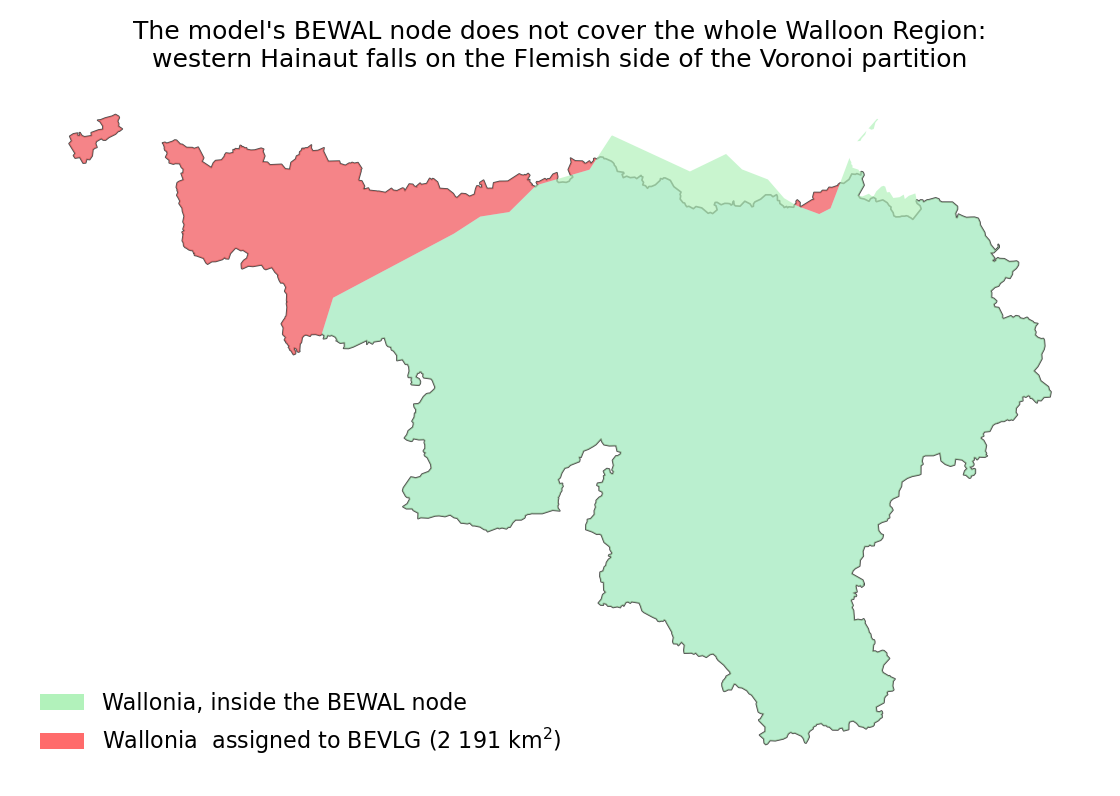
\includegraphics[width=\linewidth]{figures/region_mismatch.png}
\caption{Wallonia and the model's \texttt{BEWAL} node. The red area is Walloon
territory attributed to \texttt{BEVLG} by the Voronoi partition.}
\label{fig:mismatch}
\end{figure}

\finding{Any Walloon potential reported to the administration must state which
of the two regions it refers to. A cap derived from the administrative Region
and applied to the \texttt{BEWAL} node silently grants Wallonia the resource of
land the model has already given to Flanders --- and conversely, a
\texttt{BEWAL} figure understates what Wallonia as a Region can host. Both are
reported throughout this document.}

\caveat{This is a defect of the model's regionalisation, not of the potential
calculation, and it affects every Walloon quantity in PyPSA-Wal that is
land-based --- solar ground-mounted potential and biomass among them. Fixing it
means correcting the busmap, which is out of scope here but should be
raised separately.}

% =====================================================================
\section{Results}
% =====================================================================

\subsection{How much land each rule removes}

Scenarios \texttt{S1}--\texttt{S5} are cumulative: each adds layers to the
previous one, so the difference between two consecutive rows is the cost of the
rules that were added. \texttt{S0} is \emph{not} part of that sequence --- it is
PyPSA-Eur's own specification, a different constraint set rather than a subset
of \texttt{S1} --- and it is shown apart in the table and in grey in the figure.
It is larger than \texttt{S5} but smaller than \texttt{S1}, because it applies a
\SI{1}{\kilo\metre} urban buffer and Natura~2000 that \texttt{S1} does not,
while ignoring the zoning, setback, landscape and hazard rules that \texttt{S1}
and its successors impose.

\finding{The Walloon plan de secteur on its own leaves
\ZoningOnly{}~\si{\square\kilo\metre} admissible. Adding the setbacks of the
cadre de référence --- \HabitatSetback{}~m from habitat zones and
\SI{400}{\metre} from every dwelling --- removes
\SetbackRemoved{}~\si{\square\kilo\metre}, or \SetbackCut{}\,\% of it, in a
single step. Everything that follows (protected areas, landscape perimeters,
natural hazards) together removes about a third of what is left. The Walloon
onshore-wind potential is governed by settlement pattern, not by nature
protection and not by the wind.}

\begin{figure}[htbp]\centering
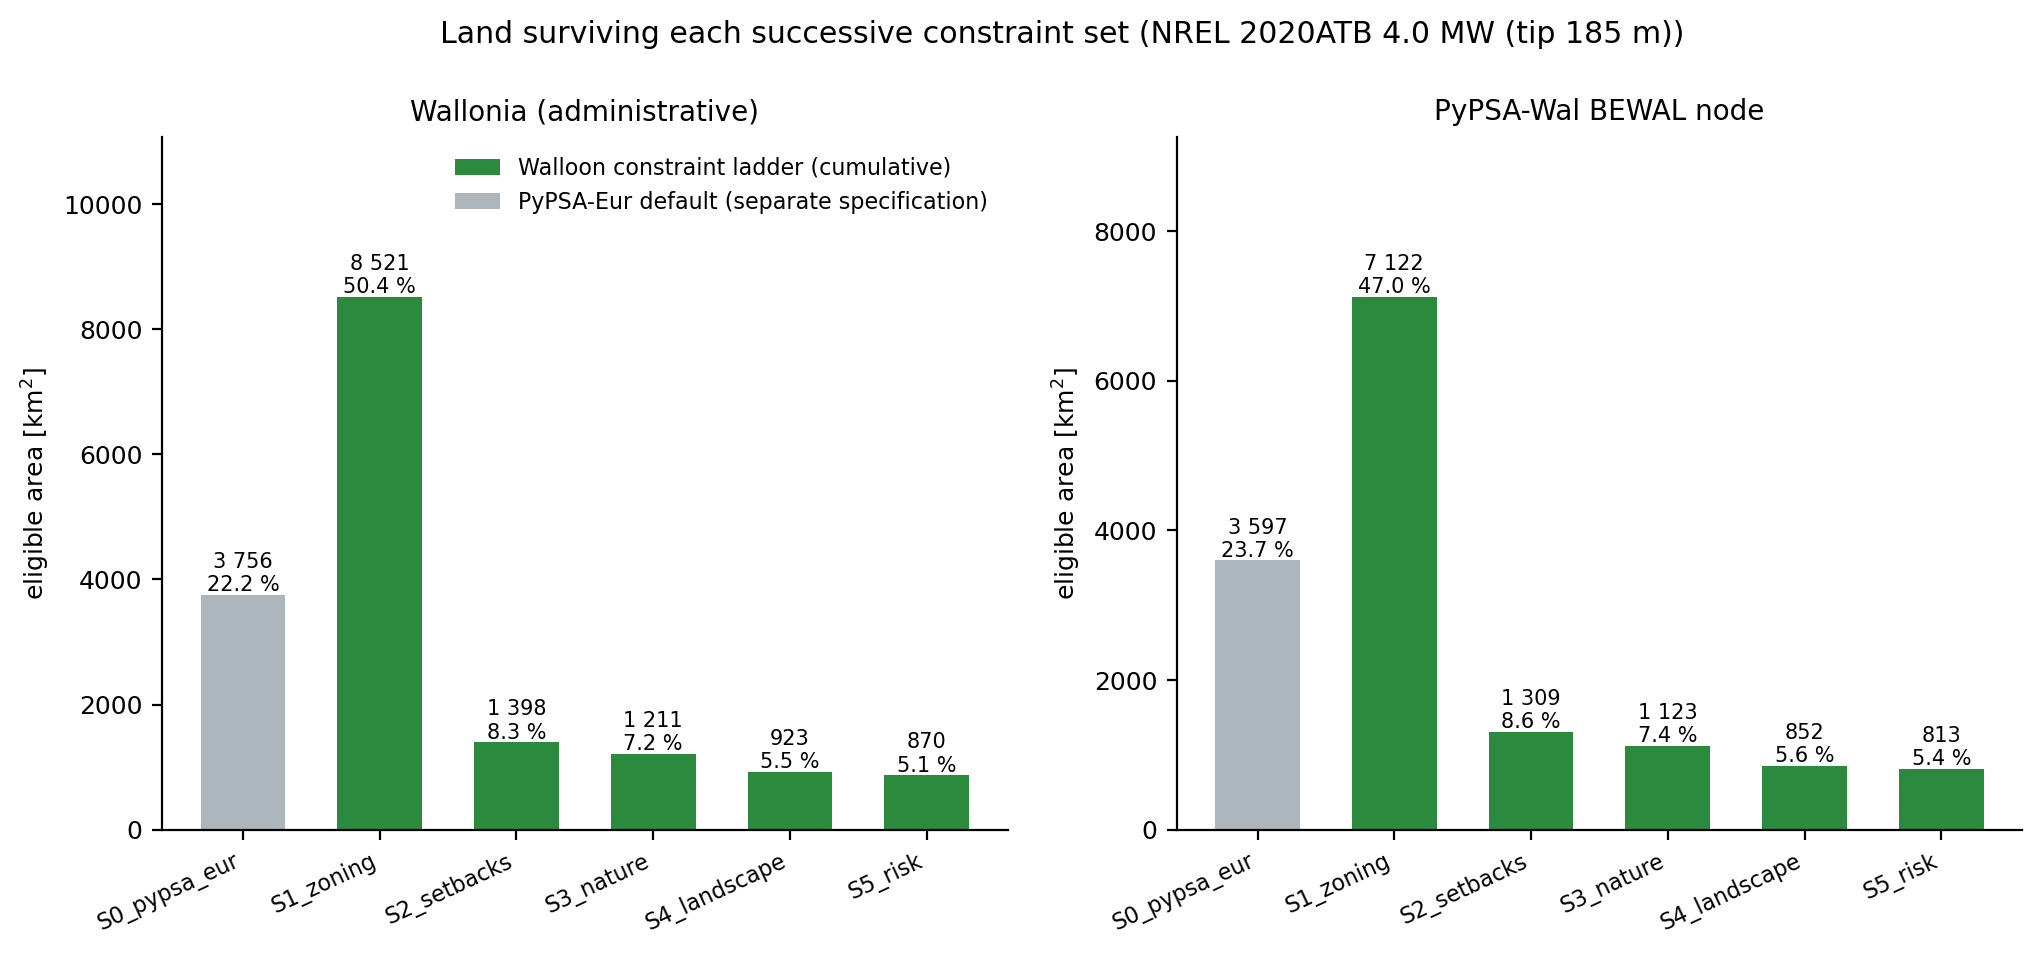
\includegraphics[width=\linewidth]{figures/waterfall.png}
\caption{Land surviving each successive constraint set, for the reference
turbine class.}
\label{fig:waterfall}
\end{figure}

\begin{table}[htbp]\centering\small
\caption{Eligible area after each constraint set.}
\label{tab:waterfall}
\begin{tabular}{lp{0.36\linewidth}rrr}
\toprule
scen. & constraint set & area [\si{\square\kilo\metre}] & share [\%] & removed [\si{\square\kilo\metre}] \\
\midrule
S0 pypsa eur & PyPSA-Eur default (CORINE + Natura 2000) & 3\,756 & 22.22 & n/a \\
S1 zoning & + plan de secteur zoning (CoDT) & 8\,521 & 50.40 & 8\,385 \\
S2 setbacks & + dwellings and infrastructure setbacks (CDR 2024) & 1\,398 & 8.27 & 7\,122 \\
S3 nature & + Natura 2000, reserves, wetlands, caves & 1\,211 & 7.16 & 187 \\
S4 landscape & + landscape protection perimeters (PIP / ADESA) & 923 & 5.46 & 288 \\
S5 risk & + flood, karst, landslide, water-capture protection & 870 & 5.14 & 54 \\
S6 servitudes & + aeronautical servitudes, slope >= 7 \%, classified sites, radar & 561 & 3.32 & 309 \\
\bottomrule
\end{tabular}
\end{table}

\begin{figure}[htbp]\centering
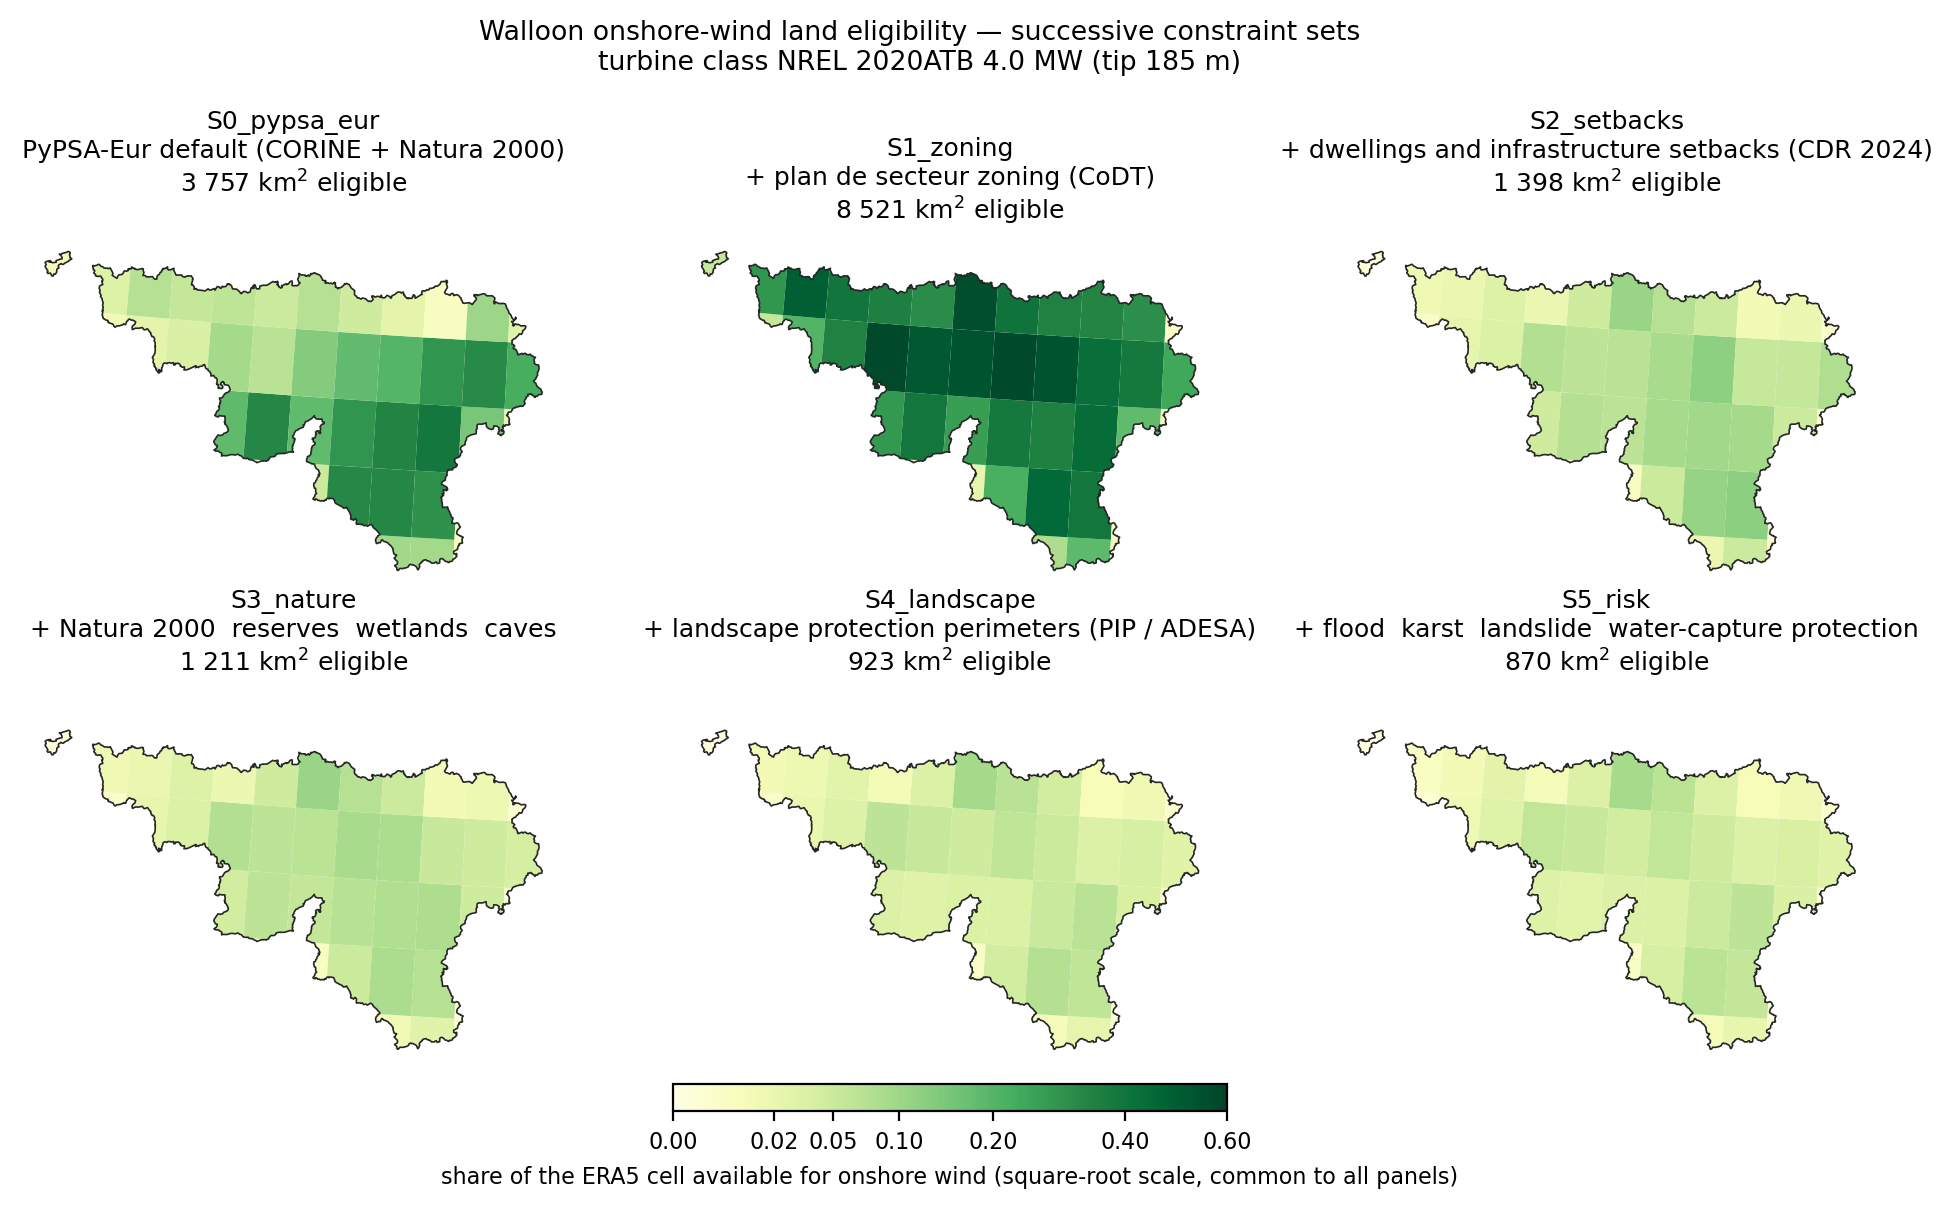
\includegraphics[width=\linewidth]{figures/map_scenarios.png}
\caption{Spatial effect of each constraint set. The shading is the share of each
ERA5 cell that survives; the ERA5 grid is $0.3^\circ$, so these panels show
\emph{where} the resource is, not the parcel-level pattern.}
\label{fig:maps}
\end{figure}

\begin{figure}[htbp]\centering
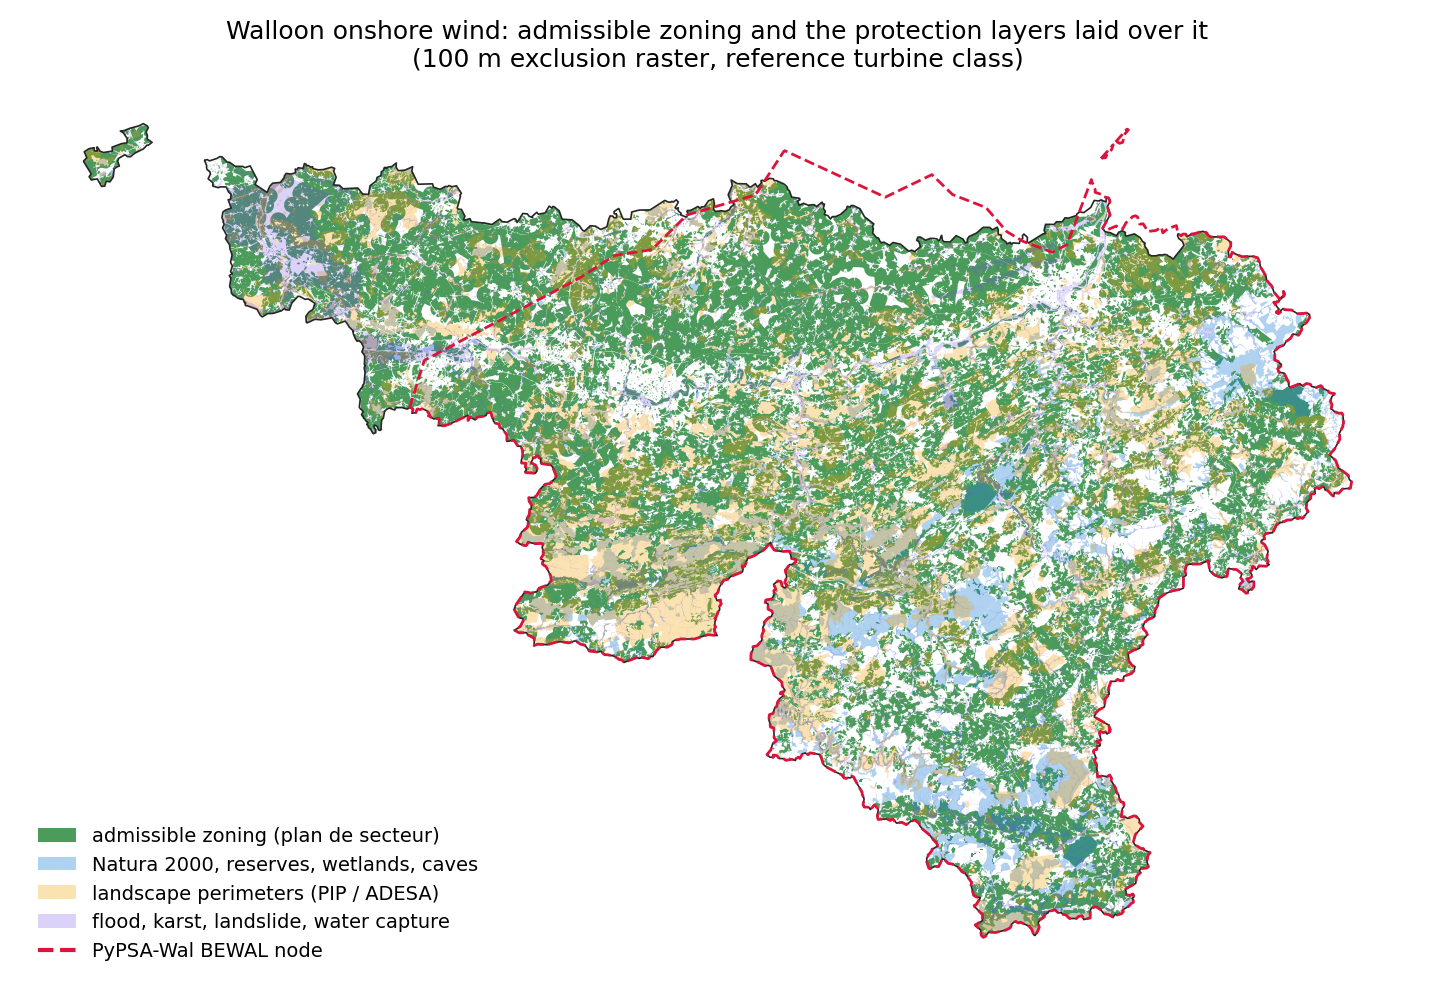
\includegraphics[width=\linewidth]{figures/map_reference.png}
\caption{The admissible plan-de-secteur envelope with the protection layers laid
over it, at the \SI{100}{\metre} resolution of the exclusion raster.}
\label{fig:reference}
\end{figure}

\begin{figure}[htbp]\centering
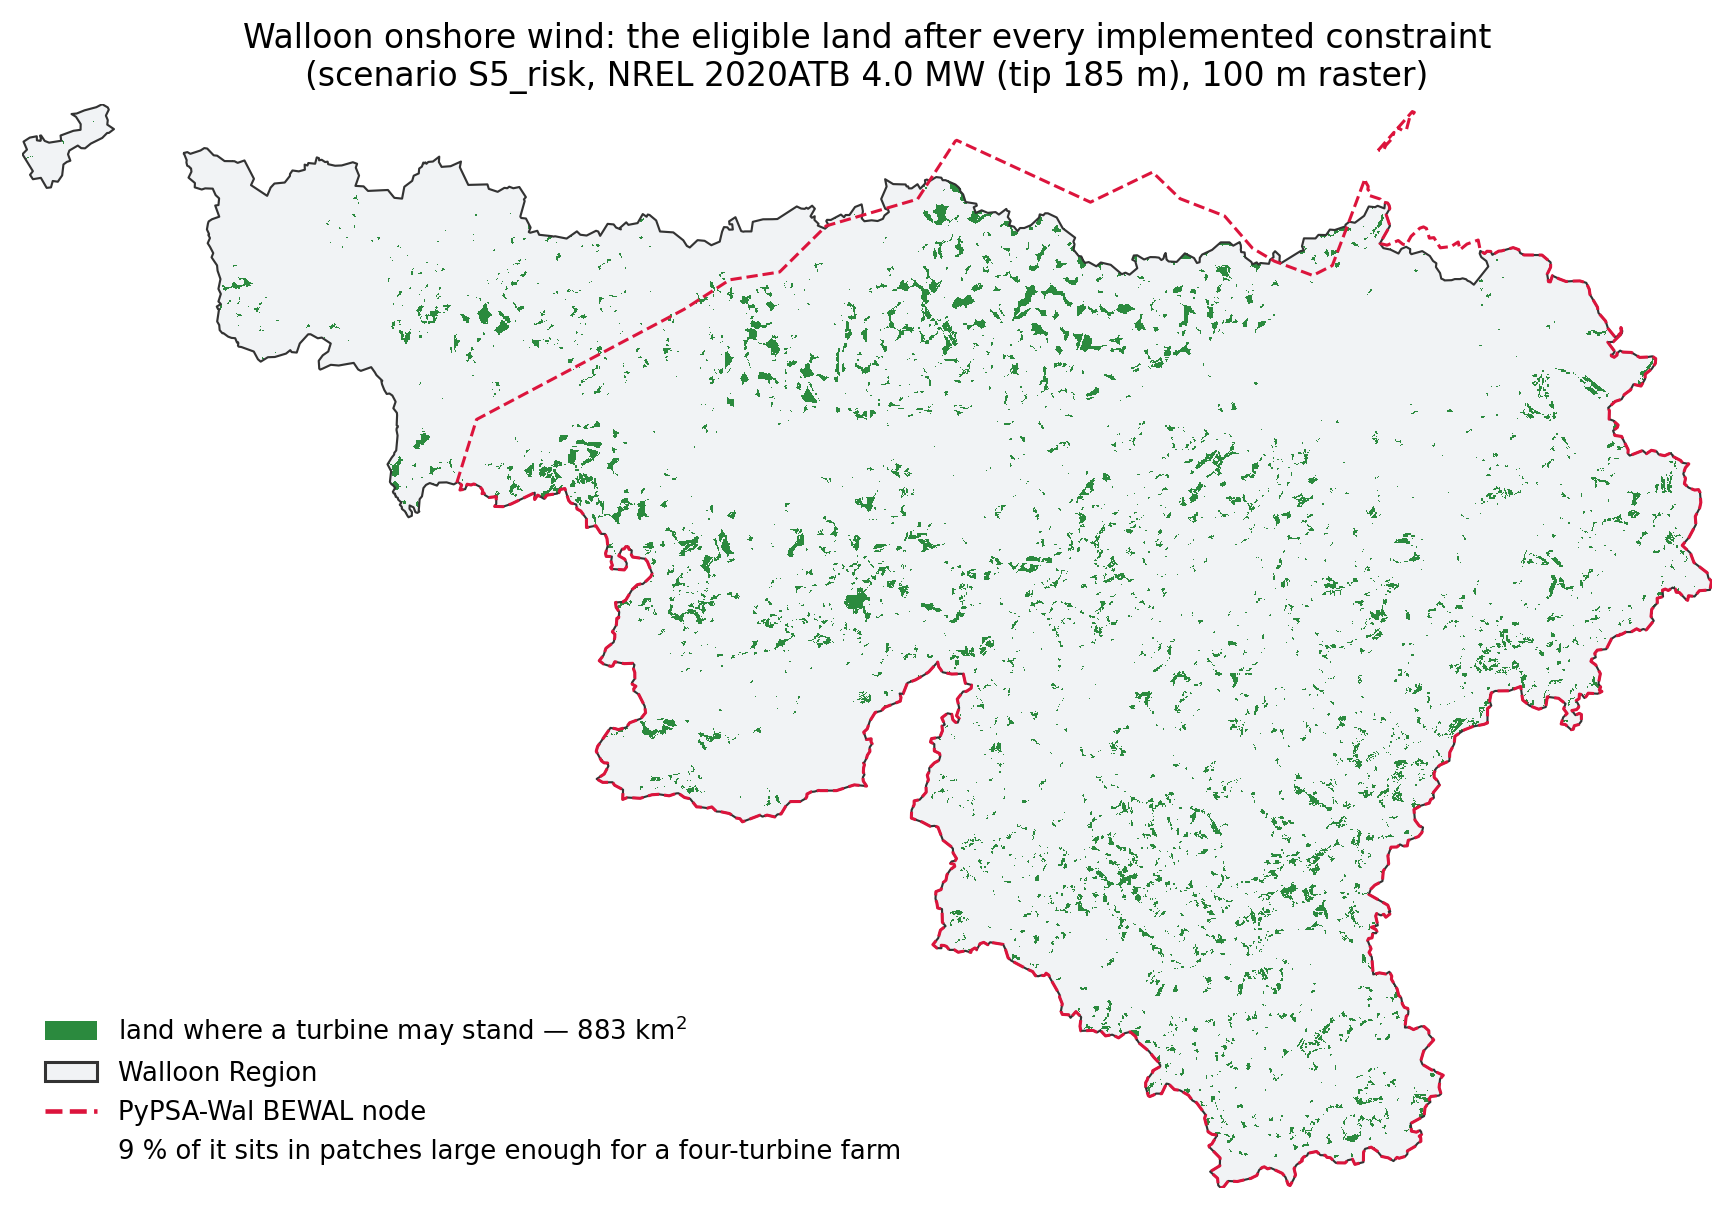
\includegraphics[width=\linewidth]{figures/map_eligible.png}
\caption{The answer, at \SI{100}{\metre} resolution: the land that survives
\emph{every} implemented constraint. This is the raster the potential is
integrated from, and it is written out as
\texttt{results/eligible\_land.tif} so it can be opened in QGIS and checked
parcel by parcel.}
\label{fig:eligible}
\end{figure}

\subsection{Installable capacity}

\begin{table}[htbp]\centering\small
\caption{Reference scenario \refScenario{} across turbine classes and capacity
densities. \emph{derived} is $P_{\mathrm{nom}}/(5D\times7D)$; \emph{pypsa eur}
is PyPSA-Eur's \SI{3}{\mega\watt\per\square\kilo\metre}; \emph{dense} is a
$4D\times6D$ upper bound.}
\label{tab:sensitivity}
\begin{tabular}{llrrrrr}
\toprule
turbine & density & [\si{\mega\watt\per\square\kilo\metre}] & area [\si{\square\kilo\metre}] & $P$ [\si{\mega\watt}] & FLH [\si{\hour}] & $E$ [\si{\tera\watt\hour}] \\
\midrule
V112 / 3.0 MW (tip 136 m) & dense & 8.00 & 611 & 4\,890 & 2\,470 & 12.1 \\
 & derived & 6.83 & 611 & 4\,176 & 2\,470 & 10.3 \\
 & pypsa eur & 3.00 & 611 & 1\,834 & 2\,470 & 4.5 \\
\midrule
NREL 2020ATB 4.0 MW (tip 185 m) & dense & 8.00 & 561 & 4\,487 & 3\,264 & 14.6 \\
 & derived & 5.08 & 561 & 2\,849 & 3\,264 & 9.3 \\
 & pypsa eur & 3.00 & 561 & 1\,683 & 3\,264 & 5.5 \\
\midrule
NREL 2020ATB 5.5 MW (tip 208 m) & dense & 8.00 & 534 & 4\,273 & 3\,337 & 14.3 \\
 & derived & 5.13 & 534 & 2\,740 & 3\,337 & 9.1 \\
 & pypsa eur & 3.00 & 534 & 1\,602 & 3\,337 & 5.3 \\
\bottomrule
\end{tabular}
\end{table}

\begin{figure}[htbp]\centering
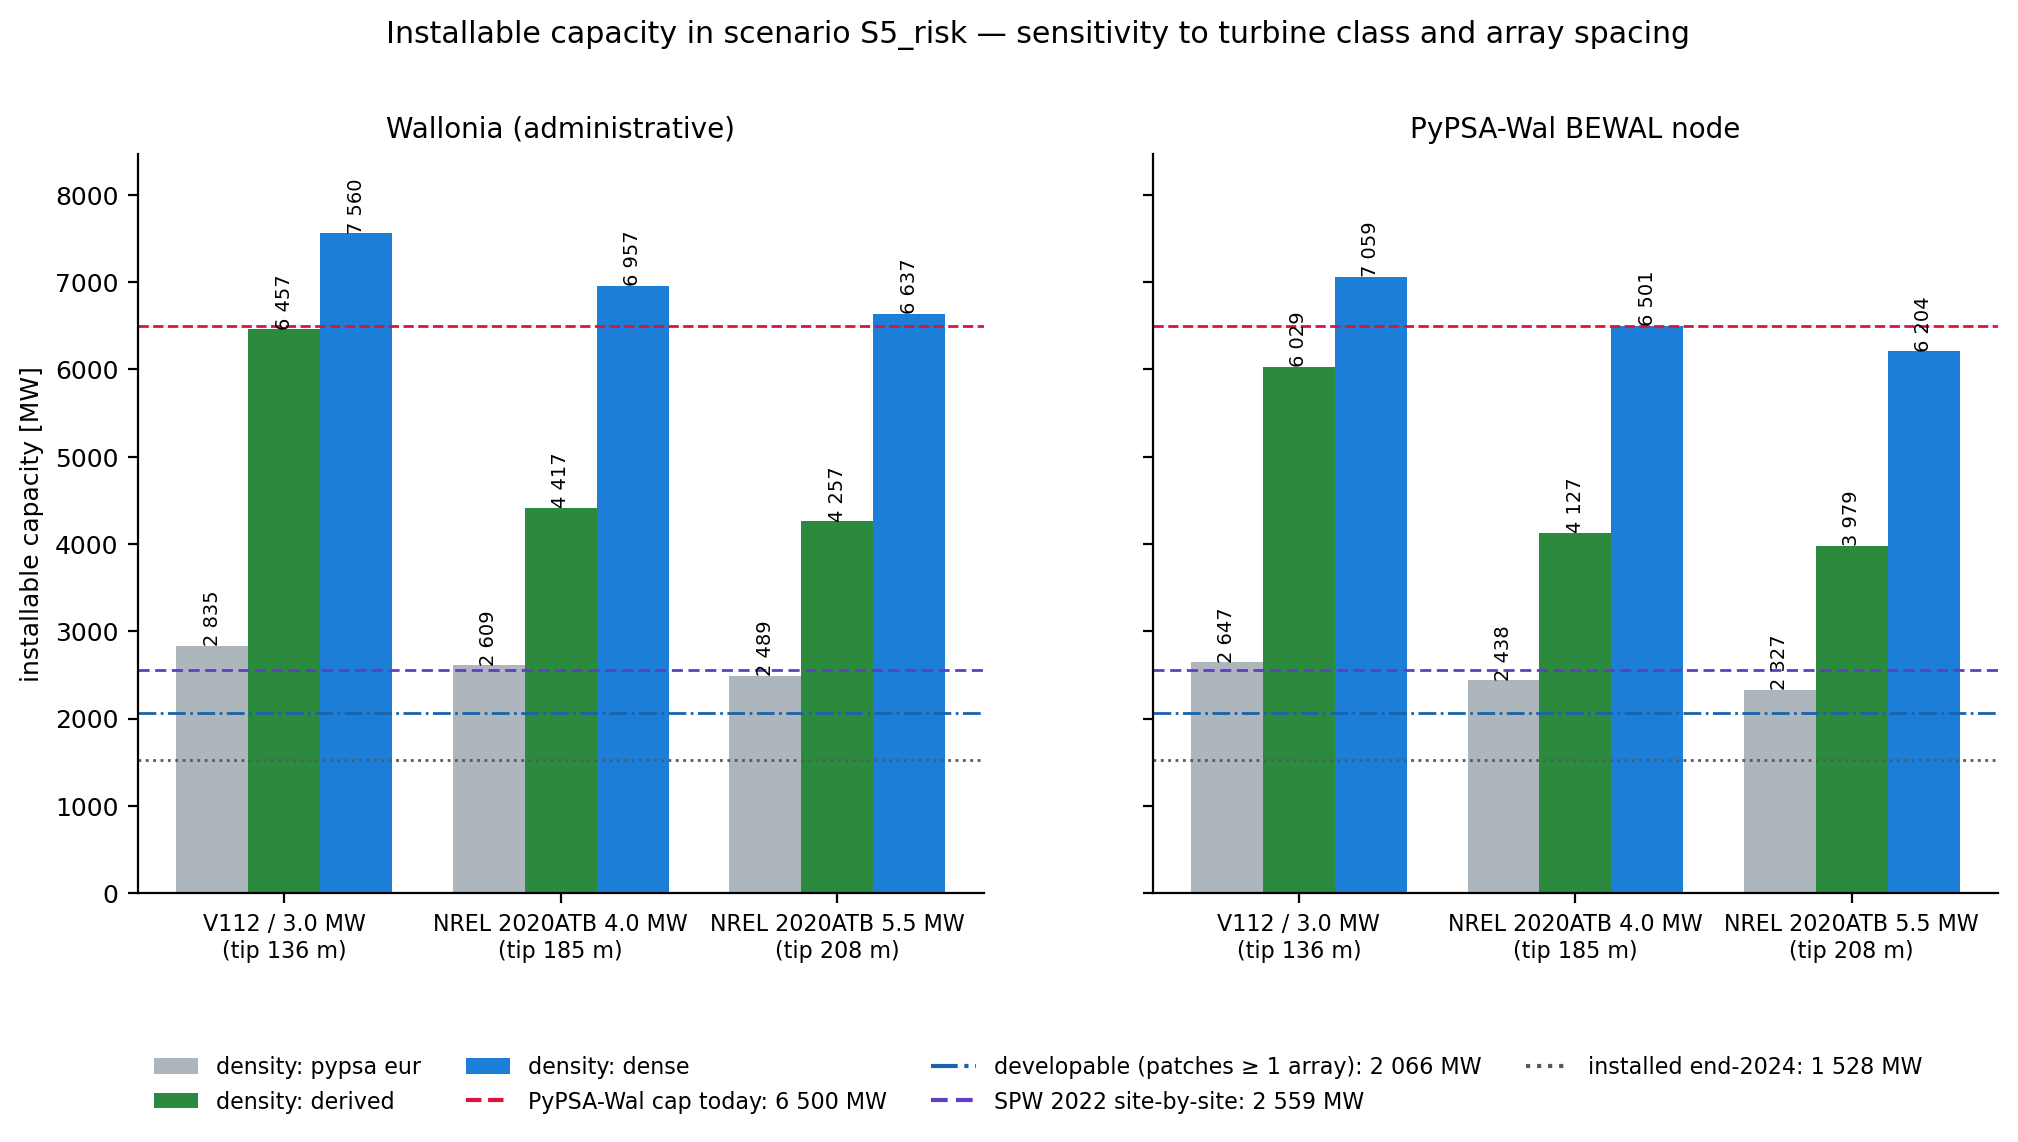
\includegraphics[width=\linewidth]{figures/sensitivity.png}
\caption{Installable capacity in the reference scenario, by turbine class and
array spacing.}
\label{fig:sensitivity}
\end{figure}

\paragraph{Turbine class barely moves the energy, only the capacity.} Across the
three classes the energy yield per square kilometre of eligible land is
\EnergyDensityLow{}--\EnergyDensityHigh{}~GWh/\si{\square\kilo\metre}, a spread
of a few per cent, while the installed capacity on the same land spans
\SI{4257}{\mega\watt} to \SI{6457}{\mega\watt}. That is the expected physics:
at fixed rotor-diameter spacing the swept area per square kilometre is a
constant, so a low-specific-power machine trades megawatts for full-load hours
at roughly constant energy. It also means the choice of turbine class is close
to irrelevant for what the model actually needs from this study --- annual
energy --- and decisive for the headline capacity number, which is a reason to
report both.

\subsection{The eligible land is fragmented, and that is half the answer}
\label{sec:fragmentation}

Figure~\ref{fig:eligible} shows why an area figure alone is not enough. The
\AdminEligible{}~\si{\square\kilo\metre} that survive are not a few large
blocks; they are \NPatches{} disconnected patches with a median size of
\MedianPatch{}~ha and a largest of \LargestPatch{}~\si{\square\kilo\metre}.
Multiplying that area by a capacity density assumes an array at
$5D\times7D$ spacing --- \Footprint{}~\si{\square\kilo\metre} per machine for
the reference class --- which a three-hectare patch cannot hold.

Screening the patches by size gives a bracket:

\begin{table}[htbp]\centering\small
\caption{Installable capacity under three developability screens, reference
scenario and turbine class, administrative Wallonia, at
\refDensity{}~MW/\si{\square\kilo\metre}.}
\label{tab:developable}
\begin{tabular}{lrrr}
\toprule
screen & area [\si{\square\kilo\metre}] & share & $p_{\mathrm{nom,max}}$ [\si{\mega\watt}] \\
\midrule
all eligible land & \AdminEligible{} & 100\,\% & \DevAllMW{} \\
patches $\geq$ one turbine array & \DevOneKm{} & \DevOnePct{}\,\% & \DevOneMW{} \\
patches $\geq$ four turbine arrays & \DevFourKm{} & \DevFourPct{}\,\% & \DevFourMW{} \\
\bottomrule
\end{tabular}
\end{table}

Neither end of the bracket is the answer. The unfiltered figure counts land no
machine could occupy. The four-array filter is too strict in the other
direction: a wind farm's turbines do not have to sit inside one contiguous
eligible polygon --- they can straddle a road, a hedgerow or a setback sliver,
and the access tracks and cabling that join them cross ineligible land as a
matter of course. The \SI{500}{\metre}-scale gaps that fragment this raster are
mostly setback slivers, not obstacles.

\finding{The developability screen is what reconciles this study with the
Region's own. Filtering to patches that can hold at least one turbine array
gives \DevOneMW{}~MW, against the \SI{2559}{\mega\watt} implied by the 457
potential turbines of the 2022 SPW/Gembloux site-by-site simulation --- two
methods with different data and different logic landing within 20\,\% of each
other. That agreement is the strongest evidence in this report that the order
of magnitude is right, and it puts the credible technical potential at
\textbf{2--4.5~GW}, not at \CapTodayGW{}~GW.}

\subsection{Against the numbers in circulation}\label{sec:comparison}

\begin{table}[htbp]\centering\small
\caption{This study against the figures currently used or published.}
\label{tab:comparison}
\begin{tabular}{p{0.32\linewidth}p{0.34\linewidth}rr}
\toprule
source & basis & $P$ [\si{\mega\watt}] & $E$ [\si{\tera\watt\hour}] \\
\midrule
PyPSA-Wal today (input\_parameters\_for\_models.csv) & PNEC wallon / EDORA, expert judgement & 6\,500 & 21.19 \\
PyPSA-Eur default land eligibility & this study, scenario S0, area x 3 MW/km2 & 19\,079 & 61.62 \\
BREGILAB / VITO Dynamic Energy Atlas & Clymans et al. 2022, V112 at 5 D, free allocation, gross & 11\,400 & 18.20 \\
BREGILAB's rules on this study's data & this study, emulation of the WTN scenario, V112 at 5 D & 25\,087 & -- \\
Walloon constraint set, area x density & this study, S6\_servitudes, 5.08 MW/km2 & 2\,136 & 6.96 \\
Walloon constraint set, free allocation & this study, S6\_servitudes, 750 m between machines, no grouping rule & 11\,460 & 37.36 \\
Walloon constraint set, parks of 4 or more & this study, S6\_servitudes, no landscape rule & 8\,648 & 28.19 \\
Walloon constraint set, parks and open horizon & this study, S6\_servitudes, gross reference & 6\,480 & 21.12 \\
Walloon constraint set, machines placed, residual allowance & this study, central allowance for the families with no geometry & 4\,957 & 16.16 \\
SPW/Gembloux favourable-zone update 2022, '180 m' case & site-by-site simulation, additional potential only & -- & 3.96 \\
Installed fleet, end 2024 & EDORA / Renouvelle & 1\,528 & -- \\
PNEC / PACE 2030 onshore-wind target & Walloon Government & -- & 6.20 \\
\bottomrule
\end{tabular}
\end{table}

Three comparisons deserve comment.

\paragraph{Against the 2022 SPW/Gembloux favourable-zone update.}
That study reports \SpwStrictArea{}~\si{\square\kilo\metre} of \emph{zones
favorables strictes} and \SpwEnlargedArea{}~\si{\square\kilo\metre} of
\emph{zones favorables élargies} for its ``180~m'' case, and
\SpwNewGWh{}~GWh/yr of \emph{additional} production from
457 potential turbines. Two differences are structural and both are expected:

\begin{itemize}
  \item It applies constraints this workflow cannot --- aviation and defence
    radar, priority bird zones, classified sites, the $7\,\%$ slope criterion
    --- so its eligible area is smaller than what is reported here for the same
    nominal rule set.
  \item It then places individual machines and screens them against landscape
    inter-distance and encirclement criteria, and it counts only \emph{new}
    capacity, excluding the footprint of the standing fleet.
\end{itemize}

The two numbers therefore bracket the answer from opposite sides: this study is
an upper bound on eligible land under the constraints it can represent; the 2022
study is a lower bound reflecting a full permitting screen on a fixed turbine
layout. Both are far below \CapToday{}~MW.

\paragraph{Against the PNEC/PACE target.} The Walloon 2030 onshore-wind target
is \TargetGWh{}~GWh/yr, revised upward from the 4\,600~GWh/yr of the 2019 plan
--- which is the figure the 2022 favourable-zone update was benchmarked
against, and which it concluded was reachable. The reference case here yields
\AdminEnergy{}~TWh/yr for the administrative Region at \AdminFlh{} full-load
hours on an all-new fleet occupying every eligible parcel, which is an envelope
and not a forecast.

\paragraph{Against the model's own cap.} \CapToday{}~MW against the reference
case's \ModelPnom{}~MW is a factor of \CapOverstatement{}. But the reference
case is one point in a range, and \CapToday{}~MW is inside it: the same eligible
land supports \ModelRangeHigh{}~MW at the densest packing considered, and
\SI{6029}{\mega\watt} on a V112-class fleet at conventional $5D\times7D$
spacing. The honest statement is therefore narrower than "the cap is too high''.

\finding{\CapToday{}~MW is reachable on the \emph{unfiltered} eligible land, but
only at a capacity density around \SI{6.8}{\mega\watt\per\square\kilo\metre},
only if the four unimplemented constraint families of §\ref{sec:open} --- radar,
slope, priority bird zones, classified sites --- turn out to cost little, and
only if every fragment of eligible land counts --- including the
\SI{54}{\percent} of it that sits in patches too small to hold a single turbine
array (§\ref{sec:fragmentation}). Once the developability screen is applied, the two
independent methods available --- this one and the Region's own 2022
site-by-site simulation --- agree on 2--4.5~GW.}

\subsection{Full-load hours}

The capacity factor is computed on the 2013 ERA5/SARAH-3 cutout with the same
layout weighting PyPSA-Eur uses. For the administrative Region the reference
case gives \AdminFlh{}~h; for \texttt{BEWAL}, \ModelFlh{}~h.

Those are high numbers, and the reason is the machine, not the method. The
reference class is an NREL~2020~ATB \SI{4}{\mega\watt} turbine with a
\SI{150}{\metre} rotor --- a specific power of \SI{226}{\watt\per\square\metre},
against \SI{305}{\watt\per\square\metre} for the V112 PyPSA-Eur uses by default
--- on a \SI{110}{\metre} hub instead of \SI{80}{\metre}. Low-specific-power
machines on tall towers are exactly what raises full-load hours, and it is why
the same workflow returns \VOneTwelveFlh{}~h when the V112 is substituted into
the same eligible land (Table~\ref{tab:sensitivity}). The V112 number is the one
that reconciles with §\ref{sec:validation} and with the model's own resource.

\caveat{These are \emph{new-turbine} full-load hours applied to a hypothetical
all-new fleet, and they are not comparable with the 1\,885~h TIMES-WAL uses for
the blended existing fleet, nor with what the standing Walloon fleet actually
delivers. That discrepancy is analysed in
\texttt{docs/renewable-potentials.md}~§10 and is not re-opened here. The
relevant point for this report is that a \emph{technical potential} is by
definition about what could be built from now on, so the new-turbine figure is
the right one in this context.}

\caveat{Only the 2013 weather year is available on this machine. The Walloon
onshore-wind resource in 2013 is about 5\,\% \emph{better} than in 2010, the
year the main model runs use (\texttt{docs/renewable-potentials.md}~§10.1).
Capacity is unaffected --- it depends only on eligible area --- but the energy
column is optimistic by roughly that margin relative to a 2010 run.}

% =====================================================================
\section{Assumptions}
% =====================================================================

The result depends on the following choices. Each is a config entry and each can
be varied.

\begin{description}
  \item[Capacity density.] The reference is \refDensity{}~MW/\si{\square\kilo\metre},
    derived from the reference turbine at $5D$ crosswind $\times$ $7D$ downwind
    spacing. This is a \emph{technical} density on land that has already been
    filtered to genuinely developable parcels; PyPSA-Eur's
    \SI{3}{\mega\watt\per\square\kilo\metre} is a deliberately conservative
    continental prior applied to much less filtered land. Both are reported.
  \item[Array spacing.] $5D\times7D$ is conventional for a prevailing-wind
    regime. A $4D\times6D$ packing raises the density by about 45\,\%.
  \item[Habitat setback rule.] The 2024 framework ($500+H/2$). The 2013 rule
    ($4H$) is available and is more restrictive for machines above
    \SI{250}{\metre} tip height --- i.e. for every class considered here.
  \item[Scattered dwellings.] \SI{400}{\metre} around every ICAR address point.
    The address layer includes non-residential buildings (schools, churches,
    commercial premises), so this is mildly conservative; the 2022 SPW study
    makes the same approximation and notes the same caveat.
  \item[Broad-leaved / coniferous split.] Taken from CORINE at
    \SI{250}{\metre}; mixed stands are counted as broad-leaved. The Region's
    own CARTOFOR species-proportion map would be better and is the natural
    upgrade (§\ref{sec:open}).
  \item[Runoff flood hazard excluded from the flood layer.] The
    \emph{ruissellement} hazard layer holds 5.2~million polygons and maps a
    thin-sheet phenomenon that does not preclude a turbine foundation. The
    overflow extent at the extreme return period is used instead.
  \item[Geometry generalisation.] Heavy polygon layers are requested from the
    server with \SI{25}{\metre} generalisation --- a quarter of the exclusion
    raster cell, so it cannot change the aggregate.
  \item[Existing wind farms are not excluded.] The result is a \emph{gross}
    potential: the standing \Installed{}~MW occupies land that is counted as
    available. This is the right convention for \texttt{p\_nom\_max}, which is a
    cap on the \emph{total} fleet, not on additions.
  \item[Every fragment of eligible land is counted in the headline figure.]
    The developability screen of §\ref{sec:fragmentation} is reported
    separately rather than applied, because its cut-off is a judgement.
  \item[No grid-connection or economic screen.] Distance to the HV network,
    connection cost and wind-speed profitability thresholds are not applied. The
    2022 SPW study applies a wind-resource threshold; this one does not, so its
    eligible area is larger on that count too.
\end{description}

% =====================================================================
\section{Open questions}\label{sec:open}
% =====================================================================

These are the gaps that stand between this analysis and one that the
administration could adopt without qualification. They are listed in the order
in which they would change the number.

\begin{enumerate}
  \item \textbf{Aviation and defence radar exclusions are missing, and they are
    large.} In Belgium the secondary-radar exclusion radius is
    of the order of \SI{10}{\kilo\metre} with a study zone out to
    \SI{16}{\kilo\metre}, plus
    beacon and military-airspace constraints covering the whole territory.
    Neither skeyes nor Defence publishes the geometry as open data. Obtaining
    those layers --- they exist, the SPW favourable-zone map uses them --- is
    the single most important improvement, and it can only reduce the potential.
    \emph{Action: request the layers from SPW Énergie or from the authors of the
    favourable-zone cartography.}
  \item \textbf{The $7\,\%$ slope criterion is not applied.} The 2013 Walloon
    map excludes slopes above $7\,\%$ as technically incompatible. Only the
    $>30^\circ$ layer is public here. On a \SI{1}{\metre} LiDAR model a $7\,\%$
    threshold is very restrictive; on a \SI{30}{\metre} DEM it is a different
    quantity entirely. The Region's own slope raster should be used, at a
    resolution the two studies agree on. \emph{Direction: reduces the potential,
    most in the Ardennes.}
  \item \textbf{Priority ornithological zones and classified sites are
    missing.} The DEMNA high-priority bird layer and the classified-site
    inventory are integral exclusions in the Walloon method. \emph{Direction:
    reduces.}
  \item \textbf{Partial constraints are not modelled at all.} The Walloon method
    distinguishes integral from \emph{partial} exclusions (medium-priority bird
    zones, bat interest zones, migration corridors, the principal ecological
    structure, radar study zones at 8--16~km) and applies a 25\,\% success rate
    to turbines falling in them. Implementing them would require a site-level
    model rather than an area calculation. \emph{Direction: reduces.}
  \item \textbf{Landscape inter-distance and encirclement are not modelled.}
    These are the criteria that cut the 2022 study from 1\,323 simulated
    turbines to 457 potential ones. An area-based method cannot represent them.
    \emph{Direction: reduces, substantially.}
  \item \textbf{The developability screen of §\ref{sec:fragmentation} is a
    proxy, and it is the widest uncertainty in this report.} Requiring a patch
    to hold a whole $5D\times7D$ array is too strict, because real turbines
    straddle setback slivers and their access tracks cross ineligible land;
    counting every fragment is too lax. The bracket is \DevOneMW{}--\AdminPnom{}~MW
    and the right answer is inside it. Closing it properly means placing
    machines, i.e. doing what the 2022 study did --- which is the natural next
    step if the cabinet wants a single number rather than a range.
    \emph{Direction: the true value is below the unscreened figure.}
  \item \textbf{The CORINE forest split should be replaced by CARTOFOR.} The
    Region's own species-proportion map, at the resolution the plan-de-secteur
    forest polygons deserve, would remove a real source of error in the
    single constraint that matters most. \emph{Direction: unknown.}
  \item \textbf{The model's BEWAL node should be corrected.} See
    Section~\ref{sec:region}. Until it is, the Walloon cap is being applied to a
    region that is \modelCoverage{}\,\% of Wallonia.
  \item \textbf{Repowering is not represented.} EDORA's 3.8~GW additional
    potential by 2050 explicitly includes repowering of existing sites with
    larger machines. A land-eligibility study measures the envelope, not the
    turnover of the fleet inside it; the two are complementary, and the
    difference between them is part of why \CapToday{}~MW and \ModelPnom{}~MW
    differ.
  \item \textbf{The weather year is 2013, not 2010.} Only capacity factors are
    affected; see §\ref{sec:comparison}.
  \item \textbf{Should \texttt{p\_nom\_max} be a technical or a deployment
    limit?} PyPSA-Wal already carries a build-rate limit and a 2030 corridor
    (\texttt{docs/renewable-potentials.md}~§3--4) to represent deployment.
    If those are doing their job, \texttt{p\_nom\_max} should be the technical
    potential and the present \CapToday{}~MW is the wrong kind of number in the
    wrong slot. That is a modelling decision, not a GIS one.
\end{enumerate}

% =====================================================================
\section{What we recommend deciding}
% =====================================================================

\begin{enumerate}
  \item \textbf{Do not change \texttt{p\_nom\_max} yet.} The missing radar and
    slope layers all push in the same direction --- downwards --- so the figure
    reported here is an upper bound on an upper bound. Changing the cap on the
    basis of an incomplete constraint set would replace one unsourced number
    with another. What can be done now, at no risk, is to \emph{document} the
    existing \CapToday{}~MW with the land basis and capacity density that make
    it arithmetically reachable
    (\AdminEligible{}~\si{\square\kilo\metre} at \SI{6.8}{\mega\watt\per\square\kilo\metre}),
    so the administration can contest a number rather than a citation.
  \item \textbf{Request the missing layers} (item~1 and item~2 of
    §\ref{sec:open}) from SPW Énergie. They exist; this is an administrative
    step, not a research one.
  \item \textbf{Settle the region question} (§\ref{sec:region}) before any
    number is quoted externally.
  \item \textbf{If a single number is needed, place the machines.} The
    developability bracket (§\ref{sec:fragmentation}) is the widest remaining
    uncertainty and an area method cannot close it. The eligible raster is
    written out as \texttt{results/eligible\_land.tif} precisely so that a
    siting pass can be run on it.
  \item \textbf{Decide what \texttt{p\_nom\_max} is meant to be} (item~10).
    Until that is settled the comparison between \CapToday{}~MW and
    \ModelPnom{}~MW is a category error, not a discrepancy.
\end{enumerate}

\appendix
% =====================================================================
\section{Full results}\label{sec:full}
% =====================================================================

\begin{table}[htbp]\centering\small
\caption{All scenarios, turbine classes and regions at the reference capacity
density.}
\begin{tabular}{llrrrr}
\toprule
scenario & turbine & area [\si{\square\kilo\metre}] & $P$ [\si{\mega\watt}] & FLH [\si{\hour}] & $E$ [\si{\tera\watt\hour}] \\
\midrule
S0 pypsa eur & V112 / 3.0 MW (tip 136 m) & 3\,757 & 25\,668 & 2\,442 & 62.67 \\
S1 zoning & V112 / 3.0 MW (tip 136 m) & 6\,266 & 42\,814 & 2\,464 & 105.51 \\
S2 setbacks & V112 / 3.0 MW (tip 136 m) & 1\,059 & 7\,239 & 2\,453 & 17.76 \\
S3 nature & V112 / 3.0 MW (tip 136 m) & 912 & 6\,232 & 2\,459 & 15.32 \\
S4 landscape & V112 / 3.0 MW (tip 136 m) & 716 & 4\,892 & 2\,458 & 12.03 \\
S5 risk & V112 / 3.0 MW (tip 136 m) & 680 & 4\,644 & 2\,459 & 11.42 \\
S6 servitudes & V112 / 3.0 MW (tip 136 m) & 463 & 3\,164 & 2\,467 & 7.80 \\
S0 pypsa eur & NREL 2020ATB 4.0 MW (tip 185 m) & 3\,757 & 19\,079 & 3\,230 & 61.62 \\
S1 zoning & NREL 2020ATB 4.0 MW (tip 185 m) & 6\,266 & 31\,824 & 3\,258 & 103.68 \\
S2 setbacks & NREL 2020ATB 4.0 MW (tip 185 m) & 973 & 4\,943 & 3\,243 & 16.03 \\
S3 nature & NREL 2020ATB 4.0 MW (tip 185 m) & 831 & 4\,221 & 3\,250 & 13.72 \\
S4 landscape & NREL 2020ATB 4.0 MW (tip 185 m) & 651 & 3\,305 & 3\,251 & 10.75 \\
S5 risk & NREL 2020ATB 4.0 MW (tip 185 m) & 618 & 3\,140 & 3\,252 & 10.21 \\
S6 servitudes & NREL 2020ATB 4.0 MW (tip 185 m) & 420 & 2\,136 & 3\,260 & 6.96 \\
S0 pypsa eur & NREL 2020ATB 5.5 MW (tip 208 m) & 3\,757 & 19\,275 & 3\,302 & 63.65 \\
S1 zoning & NREL 2020ATB 5.5 MW (tip 208 m) & 6\,266 & 32\,150 & 3\,332 & 107.12 \\
S2 setbacks & NREL 2020ATB 5.5 MW (tip 208 m) & 929 & 4\,768 & 3\,316 & 15.81 \\
S3 nature & NREL 2020ATB 5.5 MW (tip 208 m) & 790 & 4\,051 & 3\,323 & 13.46 \\
S4 landscape & NREL 2020ATB 5.5 MW (tip 208 m) & 617 & 3\,163 & 3\,324 & 10.52 \\
S5 risk & NREL 2020ATB 5.5 MW (tip 208 m) & 586 & 3\,007 & 3\,325 & 10.00 \\
S6 servitudes & NREL 2020ATB 5.5 MW (tip 208 m) & 398 & 2\,043 & 3\,334 & 6.81 \\
\bottomrule
\end{tabular}
\end{table}

% =====================================================================
\section{Data provenance}\label{sec:sources}
% =====================================================================

All layers below were retrieved from the ESRI-REST services of the Géoportail de
la Wallonie (\url{https://geoservices.wallonie.be}) under the CC-BY~4.0 licence.

\begin{table}[htbp]\centering\small
\caption{Source datasets, as retrieved.}
\begin{tabular}{p{0.36\linewidth}p{0.30\linewidth}rl}
\toprule
dataset & service / layer & features & retrieved \\
\midrule
Points d'adresse ICAR & DONNEES\_BASE/ICAR\_ADR\_PT/1 & 1\,512\,246 & 2026-09-22 \\
Périmètres d'intérêt paysager de l'inventaire ADESA & AMENAGEMENT\_TERRITOIRE/ADESA/1 & 1\,142 & 2026-09-22 \\
Cavités souterraines d'intérêt scientifique & FAUNE\_FLORE/CONSNAT/0 & 80 & 2026-09-22 \\
Zones inondables — débordement, période de retour extrême & EAU/ZI/2 & 39\,893 & 2026-09-22 \\
Zones de contraintes karstiques & AMENAGEMENT\_TERRITOIRE/CONTR\_KARST/0 & 449 & 2026-09-22 \\
Contraintes physiques liées aux éboulements & AMENAGEMENT\_TERRITOIRE/RISQ\_EBOULT/0 & 997 & 2026-09-22 \\
Réseau Natura 2000 — périmètres des sites en vigueur & FAUNE\_FLORE/NATURA2000/9 & 240 & 2026-09-22 \\
Plan de secteur — lignes électriques haute tension & AMENAGEMENT\_TERRITOIRE/PDS/12 & 1\,016 & 2026-09-22 \\
Plan de secteur — périmètres d'intérêt paysager & AMENAGEMENT\_TERRITOIRE/PDS/17 & 1\,456 & 2026-09-22 \\
Plan de secteur — réseau ferroviaire & AMENAGEMENT\_TERRITOIRE/PDS/11 & 911 & 2026-09-22 \\
Plan de secteur — réseau routier & AMENAGEMENT\_TERRITOIRE/PDS/9 & 5\,420 & 2026-09-22 \\
Plan de secteur — voies navigables & AMENAGEMENT\_TERRITOIRE/PDS/13 & 1 & 2026-09-22 \\
Plan de secteur — zones d'affectation & AMENAGEMENT\_TERRITOIRE/PDS/22 & 43\,797 & 2026-09-22 \\
Réserves naturelles agréées & FAUNE\_FLORE/CONSNAT/3 & 264 & 2026-09-22 \\
Réserves naturelles domaniales & FAUNE\_FLORE/CONSNAT/2 & 306 & 2026-09-22 \\
Réserves forestières & FAUNE\_FLORE/CONSNAT/1 & 20 & 2026-09-22 \\
Versants supérieurs à 30 degrés & AMENAGEMENT\_TERRITOIRE/RISQ\_EBOULT/1 & 2\,834 & 2026-09-22 \\
Zones de prévention rapprochée (IIa) des captages & EAU/PROTECT\_CAPT/2 & 736 & 2026-09-22 \\
Zones humides d'intérêt biologique & FAUNE\_FLORE/CONSNAT/4 & 73 & 2026-09-22 \\
\bottomrule
\end{tabular}
\end{table}

\medskip\noindent
Additional inputs: ERA5/SARAH-3 \texttt{atlite} cutout for 2013 (Copernicus);
CORINE Land Cover 2006 at \SI{250}{\metre}, PyPSA-Eur data bundle; NUTS-3 shapes
and the PyPSA-Wal \texttt{BEWAL} onshore region, PyPSA-Eur resources; turbine
power curves from the \texttt{atlite} library (Vestas, NREL 2020~ATB).

\end{document}
